\documentclass[11pt,a4paper]{scrartcl}

% ===================== PACKAGES =====================
\usepackage[british,UKenglish,USenglish,english,american]{babel}
\usepackage[tmargin=1in, bmargin=1in, lmargin=0.75in, rmargin=0.75in]{geometry}
\usepackage{tikz}
\usepackage{graphicx}
\usepackage{pgfplots}
\pgfplotsset{width=12cm, compat=1.9}
\usepackage{setspace}
\usepackage{chemmacros}
\usepackage{chemfig}
\usepackage{esint}
\usepackage{tabularray}
\usepackage{makeidx}
\usepackage{epstopdf}
\usepackage{amssymb}
\usepackage{mathrsfs}
\usepackage{bm}
\usepackage{amsmath}
\usepackage{enumitem}
\usepackage[english]{varioref}
\usepackage{lipsum}
\usepackage{fancyhdr}
\usepackage{float}
\usepackage{empheq}
\usepackage[framemethod=tikz]{mdframed}
\numberwithin{equation}{section}
\usepackage{eso-pic}
\usepackage{calc}
\usepackage{nccmath}
\usepackage{caption}
\usepackage{subcaption}
\usepackage{gensymb}
\usepackage{amsfonts, amsthm, epsfig, epstopdf, titling, url, array}
\usepackage{tabularx}
\usepackage{makecell}
\usepackage{booktabs}
\usepackage{array}
\usepackage{siunitx}
\sisetup{input-digits=0123456789\pi}
\usepackage[symbol]{footmisc}
\usepackage{xcolor}
\usepackage{multicol}
\usepackage{boondox-cal}
\usepackage{blindtext}
\usepackage{changepage}
\usepackage{nomencl}

% ===================== SI UNITS =====================
\DeclareSIUnit\atm{atm}

% ===================== PAGE STYLE =====================
\pagestyle{fancy}
\fancypagestyle{firstpage}{\rhead{}}
\fancyhead[L]{\slshape\nouppercase{\leftmark}}
\chead{}
\rhead{}
\lfoot{\textit{}}
\cfoot{-\ \thepage\ -}
\rfoot{\textit{}}
\renewcommand{\headrulewidth}{0.4pt}
\renewcommand{\footrulewidth}{0.4pt}

% ===================== MATH OPERATORS =====================
\DeclareMathOperator{\rank}{rank}
\DeclareMathOperator{\atantwo}{atan2}
\DeclareMathOperator{\spn}{span}

% ===================== COMMANDS =====================
\newcommand{\abs}[1]{\left|#1\right|}
\newcommand{\sign}{\text{sign}}
\newcommand{\centered}[1]{\begin{tabular}{@{}l@{}} #1 \end{tabular}}

% ===================== COLORS =====================
\definecolor{mycolor1}{rgb}{0.97, 0.97, 0.97}
\definecolor{mycolor2}{rgb}{0.97, 0.97, 0.97}
\definecolor{tableShade}{gray}{0.9}

% ===================== THEOREM ENVIRONMENTS =====================
\theoremstyle{it}
\newtheorem{defn}{Definition}[section]
\newtheorem{assumption}{Assumption}[section]
\newtheorem{thm}{Theorem}[section]
\newtheorem{lemma}{Lemma}[section]
\newtheorem{corollary}{Corollary}[section]
\theoremstyle{definition}
\newtheorem{example}{Example}[section]

% ===================== CUSTOM ENVIRONMENTS =====================
\newenvironment{myitemize_1}{
	\begin{itemize}[topsep=0pt]
		\setlength{\topsep}{2pt}
		\setlength{\itemsep}{2pt}
		\setlength{\parskip}{2pt}
		\setlength{\parsep}{2pt}
	}{\end{itemize}}

\newmdenv[
innerlinewidth=0.5pt,
roundcorner=4pt,
backgroundcolor=mycolor2,
linecolor=mycolor1,
innerleftmargin=6pt,
innerrightmargin=6pt,
innertopmargin=6pt,
innerbottommargin=6pt
]{mybox}

% ===================== TABLE COLUMN TYPES =====================
\newcolumntype{Y}{>{\hsize=2\hsize}X}
\newcolumntype{Z}{>{\centering\arraybackslash\hsize=0.857\hsize}X}


% ===================== SECTION DEPTH =====================
\setcounter{secnumdepth}{3}
\setcounter{tocdepth}{3}

\title{\textbf{
		\begin{LARGE}
			DPTs for 690\,V EDrive IGBT Module:
		\end{LARGE} \\[12pt]
		\begin{Large}
			Evaluation with different driver concepts.
		\end{Large}
}}
\author{\textbf{Davide Bagnara}}

\begin{document}
	\thispagestyle{firstpage}
	\begin{mybox}
		\maketitle
		\vspace{100mm}
	\end{mybox}
	\newpage
	\tableofcontents
	\listoffigures
	\listoftables
	
	
	\newpage
	\subsection*{Nomenclature}
	\begin{itemize}
		\item[--] \textbf{AFE}: AC/DC three phase active front end;
		\item[--] \textbf{Inverter}: DC/AC three phase inverter for PSM and IM electrical machines;
		\item[--] \textbf{DPT}: Double Pulse Test;
		\item[--] \textbf{FF1200R17IP5P}: Infineon module, 1200\,A\,/\,1700\,V;
		\begin{itemize}
			\item[--] maximum junction temperature $T_\text{j}^\text{max} = \SI{175}{\celsius}$;
			\item[--] \textbf{new module under evaluation};
		\end{itemize}
		\item[--] \textbf{DP650B1700}: Danfoss module, 650\,A\,/\,1700\,V;
		\begin{itemize}
			\item[--] maximum junction temperature $T_\text{j}^\text{max} = \SI{150}{\celsius}$;
			\item[--] currently employed in 690\,V EDrive applications;
		\end{itemize}
		\item[--] \textbf{FF650R17IE4}: Infineon module, 650\,A\,/\,1700\,V;
		\begin{itemize}
			\item[--] maximum junction temperature $T_\text{j}^\text{max} = \SI{150}{\celsius}$;
			\item[--] currently employed in 690\,V EDrive applications;
		\end{itemize}
		\item[--] \textbf{FF650R17IE4DB2}: Infineon module, 650\,A\,/\,1700\,V;
		\begin{itemize}
			\item[--] maximum junction temperature $T_\text{j}^\text{max} = \SI{150}{\celsius}$;
			\item[--] currently employed in 690\,V EDrive applications;
		\end{itemize}
		\item[--] \textbf{DB1.00}: driver board currently employed in series production;
		\item[--] \textbf{DB1.51}: \textbf{new driver board under evaluation};
		\item[--] $E_\text{on}$\,$\left[\si{\milli\joule}\right]$: turn-on switching energy loss;
		\item[--] $E_\text{off}$\,$\left[\si{\milli\joule}\right]$: turn-off switching energy loss;
		\item[--] $I_\text{rr}$\,$\left[\si{\ampere}\right]$: reverse recovery current at turn-on;
		\item[--] $\Delta u_\text{ce}$\,$\left[\si{\volt}\right]$: collector-emitter voltage overshoot at turn-off;
		\item[--] $I_\text{nom}^\text{inv}$\,$\left[\si{\ampere}\right]$: nominal inverter current (RMS);
		\item[--] $I_\text{max}^\text{inv}$\,$\left[\si{\ampere}\right]$: maximum overload inverter current (RMS);
		\item[--] $I_\text{load}^\text{inv}$\,$\left[\si{\ampere}\right]$: inverter load current used for power loss calculation (RMS);
		\item[--] $f_\text{pwm}^\text{inv}$\,$\left[\si{\hertz}\right]$: inverter switching frequency;
		\item[--] $\cos(\varphi)$\,$\left[-\right]$: inverter load power factor;
		\item[--] $T_\text{j}^\text{Q}$\,$\left[\si{\celsius}\right]$: IGBT junction temperature;
		\item[--] $T_\text{j}^\text{D}$\,$\left[\si{\celsius}\right]$: diode junction temperature;
		\item[--] $P_\text{c}^\text{Q}$\,$\left[\si{\watt}\right]$: IGBT conduction power loss;
		\item[--] $P_\text{c}^\text{D}$\,$\left[\si{\watt}\right]$: diode conduction power loss;
		\item[--] $P_\text{sw}^\text{Q}$\,$\left[\si{\watt}\right]$: IGBT switching power loss;
		\item[--] $P_\text{sw}^\text{D}$\,$\left[\si{\watt}\right]$: diode switching power loss;
		\item[--] $\Delta T_\text{j}^\text{Q}$\,$\left[\si{\celsius}\right]$: IGBT junction temperature ripple;
		\item[--] $\Delta T_\text{j}^\text{D}$\,$\left[\si{\celsius}\right]$: diode junction temperature ripple;
		\item[--] $R_\text{g}^\text{on}$\,$\left[\si{\ohm}\right]$: turn-on gate resistance;
		\item[--] $R_\text{g}^\text{off}$\,$\left[\si{\ohm}\right]$: turn-off gate resistance;
		\item[--] $T_\text{hs}^\text{inv}$\,$\left[\si{\celsius}\right]$: heat-sink temperature below the inverter IGBTs.
	\end{itemize}
	\newpage

	\begin{onehalfspace}
		\begin{abstract}
			\small
			\textbf{This feasibility study investigates the potential adoption of the FF1200R17IP5P (Infineon) IGBT module as an alternative to the currently used DP650B1700 (Danfoss), FF650R17IE4 (Infineon), and FF650R17IE4DB2 (Infineon) in the 690\,V EDrive platform. In parallel to a theoretical power losses evaluation a series of Double Pulse Tests (DPTs) were carried out to characterize and compare the switching behavior of the main module DP650B1700 (Danfoss series)  and FF1200R17IP5P (new Infineon) under representative operating conditions. The evaluation also covers compatibility with both the legacy DB1.00 and the updated DB1.51 driver boards, in order to assess whether any hardware changes are required for a potential transition. The results and observations from this study aim to support the suitability of the FF1200R17IP5P as a replacement for the DP650B1700, FF650R17IE4DB2, and FF650R17IE4 modules.}
		\end{abstract}



		\section{Motivations: original design versus new performance requirements}
		The EDrive 690\,V has been designed primarily for wind applications with the following
		nominal specifications:
		\begin{itemize}
			\item[--] $I_\text{nom}^\text{inv} = \SI{370}{\ampere}$;
			\item[--] $f_\text{pwm}^\text{inv} = \SI{2.5}{\kilo\hertz}$.
		\end{itemize}
		Moreover, in wind applications, overloads are always related to wind speed (wind gusts), which are
		reflected on the AFE side. Therefore, the quantity $I_\text{nom}^\text{inv}$ can also be
		assumed as the maximum inverter current, and the typical overload capability of 140\% of electrical drives here decays.
		
		\vspace{5mm}
		\noindent\textbf{Inverter Design Criteria}
		\begin{itemize}
			\item[--] $I_\text{load}^\text{inv} = \SI{370}{\ampere}$, 100\% of the nominal inverter current;
			\item[--] $f_\text{pwm}^\text{inv} = \SI{2.5}{\kilo\hertz}$;
			\item[--] $T_\text{hs}^\text{inv} = \SI{65}{\celsius}$;
			\item[--] $\cos(\varphi) = -0.8$, generator mode;
			\item[--] $f_\text{load} = \SI{15}{\hertz}$, load frequency (critical parameter for maximum junction temperature evaluation);
			\item[--] driver board DB1.00.
		\end{itemize}
		\begin{table}[H]
			\centering
			\captionsetup{width=0.75\textwidth, font=small}
			\caption{\textbf{Original Design Inverter} --- Power losses and maximum junction temperature at $I_\text{load}^\text{inv} = \SI{370}{\ampere}$, $f_\text{pwm}^\text{inv} = \SI{2.5}{\kilo\hertz}$, $T_\text{hs}^\text{inv} = \SI{65}{\celsius}$, $\cos(\varphi) = -0.8$, with DB1.00.}
			\label{}
			\renewcommand{\arraystretch}{2.0}
			\begin{tabularx}{\textwidth}{Y|Z|Z|Z|Z|Z|Z|Z}
				\hline\hline
				& $T_\text{j}^\text{Q}$ & $T_\text{j}^\text{D}$ & $P_\text{c}^\text{Q}$ & $P_\text{c}^\text{D}$ & $P_\text{sw}^\text{Q}$ & $P_\text{sw}^\text{D}$ & $\Delta T_\text{j}$ \\
				\hline
				FF650R17IE4DB2 & \SI{95}{\celsius} & \SI{102}{\celsius}  & \SI{71}{\watt} & \SI{181}{\watt}  & \SI{337}{\watt}  & \SI{127}{\watt} & \SI{19}{\celsius} \\
				\hline\hline
			\end{tabularx}
		\end{table}
		
		\vspace{5mm}
		\noindent\textbf{AFE Design Criteria}
		\begin{itemize}
			\item[--] $I_\text{load}^\text{afe} = \SI{270}{\ampere}$, 135\% of the nominal afe current;
			\item[--] $f_\text{pwm}^\text{afe} = \SI{4}{\kilo\hertz}$;, higher switching frequency for power quality constraints;
			\item[--] $T_\text{hs}^\text{afe} = \SI{65}{\celsius}$;
			\item[--] $\cos(\varphi) = 1$, worst case scenario in terms of power losses;
			\item[--] $f_\text{grid} = \SI{50}{\hertz}$, grid frequency;
			\item[--] driver board DB1.00.
		\end{itemize}
		\begin{table}[H]
			\centering
			\captionsetup{width=0.75\textwidth, font=small}
			\caption{\textbf{Original Design AFE} --- Power losses and maximum junction temperature at $I_\text{load}^\text{inv} = \SI{270}{\ampere}$, $f_\text{pwm}^\text{inv} = \SI{4}{\kilo\hertz}$, $T_\text{hs}^\text{inv} = \SI{65}{\celsius}$, $\cos(\varphi) = 1$, with DB1.00.}
			\label{}
			\renewcommand{\arraystretch}{2.0}
			\begin{tabularx}{\textwidth}{Y|Z|Z|Z|Z|Z|Z|Z}
				\hline\hline
				& $T_\text{j}^\text{Q}$ & $T_\text{j}^\text{D}$ & $P_\text{c}^\text{Q}$ & $P_\text{c}^\text{D}$ & $P_\text{sw}^\text{Q}$ & $P_\text{sw}^\text{D}$ & $\Delta T_\text{j}$ \\
				\hline
				FF650R17IE4 & \SI{97}{\celsius} & \SI{84}{\celsius}  & \SI{163}{\watt} & \SI{24}{\watt}  & \SI{397}{\watt}  & \SI{139}{\watt} & \SI{6}{\celsius} \\
				\hline\hline
			\end{tabularx}
		\end{table}

		\subsection{New performance requirements}
		\noindent\textbf{Remark:} In recent years, the increasing adoption of the LD690V in
		electrical drive applications has highlighted the need to raise the inverter overload
		current to $I_\text{max}^\text{inv} = 1.4 \times I_\text{nom}^\text{inv}$.\\

		\noindent\textbf{Remark:} The use of hard parallelization requires operating at higher
		switching frequencies, bringing the worst-case scenario to
		$f_\text{pwm}^\text{inv} = \SI{4}{\kilo\hertz}$.\\

		\noindent\textbf{Remark:} When $\cos(\varphi) > 0$, the inverter operates as a motor
		drive (first quadrant operation), which is the typical configuration for drive
		applications. In this condition, the IGBTs are more heavily loaded.\\

		\noindent\textbf{Remark:} When $\cos(\varphi) < 0$, the inverter operates as a
		generator (second quadrant operation), which is the typical configuration for wind
		applications. In this condition, the diodes are more heavily loaded.\\

		\noindent\textbf{Remark:} A general design rule requires the following condition to be
		satisfied:
		\begin{equation}
			T_\text{j}^\text{design}(t)\Big|_\text{max} \le T_\text{j}^\text{max} - \SI{50}{\celsius}.
		\end{equation}

		The requirements outlined above highlight the need for a new IGBT module for the
		LD690V, which led to the selection of the FF1200R17IP5P.

	\subsection{IGBTs behaviour under new performance requirements: theoretical calculation}
	This subsection evaluates the power losses as well as the thermal behaviour of different IGBT modules under various
	load conditions, providing a comprehensive baseline for further investigations.
	
	Analysis involve eight case scenario of load conditions, as follows.
	
	\vspace{5mm}
	\noindent\textbf{Case Scenario 1}
	\begin{itemize}
		\item[--] $I_\text{load}^\text{inv} = \SI{370}{\ampere}$, 100\% of the nominal inverter current;
		\item[--] $f_\text{pwm}^\text{inv} = \SI{4}{\kilo\hertz}$;
		\item[--] $T_\text{hs}^\text{inv} = \SI{65}{\celsius}$;
		\item[--] $\cos(\varphi) = 0.8$, drive mode;
		\item[--] $f_\text{load} = \SI{15}{\hertz}$, load frequency (critical parameter for maximum junction temperature evaluation);
		\item[--] driver board DB1.00.
	\end{itemize}
	\begin{table}[H]
		\centering
		\captionsetup{width=0.75\textwidth, font=small}
		\caption{\textbf{Case Scenario 1} --- Power losses and maximum junction temperature at $I_\text{load}^\text{inv} = \SI{370}{\ampere}$, $f_\text{pwm}^\text{inv} = \SI{4}{\kilo\hertz}$, $T_\text{hs}^\text{inv} = \SI{65}{\celsius}$, $\cos(\varphi) = 0.8$, with DB1.00.}
		\label{tab:scenario1}
		\renewcommand{\arraystretch}{2.0}
		\begin{tabularx}{\textwidth}{Y|Z|Z|Z|Z|Z|Z|Z}
			\hline\hline
			& $T_\text{j}^\text{Q}$ & $T_\text{j}^\text{D}$ & $P_\text{c}^\text{Q}$ & $P_\text{c}^\text{D}$ & $P_\text{sw}^\text{Q}$ & $P_\text{sw}^\text{D}$ & $\Delta T_\text{j}$ \\
			\hline
			FF650R17IE4    & \SI{120}{\celsius} & \SI{97}{\celsius}  & \SI{242}{\watt} & \SI{54}{\watt}  & \SI{576}{\watt}  & \SI{175}{\watt} & \SI{25}{\celsius} \\
			\hline
			FF650R17IE4DB2 & \SI{130}{\celsius} & \SI{95}{\celsius}  & \SI{245}{\watt} & \SI{50}{\watt}  & \SI{598}{\watt}  & \SI{196}{\watt} & \SI{32}{\celsius} \\
			\hline
			FF1200R17IP5P  & \SI{110}{\celsius} & \SI{83}{\celsius}  & \SI{172}{\watt} & \SI{42}{\watt}  & \SI{705}{\watt}  & \SI{170}{\watt} & \SI{18}{\celsius} \\
			\hline\hline
		\end{tabularx}
	\end{table}
	
	\vspace{5mm}
	\noindent\textbf{Case Scenario 2}
	\begin{itemize}
		\item[--] $I_\text{load}^\text{inv} = \SI{520}{\ampere}$, 140\% of the nominal inverter current;
		\item[--] $f_\text{pwm}^\text{inv} = \SI{4}{\kilo\hertz}$;
		\item[--] $T_\text{hs}^\text{inv} = \SI{65}{\celsius}$;
		\item[--] $\cos(\varphi) = 0.8$, drive mode;
		\item[--] $f_\text{load} = \SI{15}{\hertz}$, load frequency (critical parameter for maximum junction temperature evaluation);
		\item[--] driver board DB1.00.
	\end{itemize}
	\begin{table}[H]
		\centering
		\captionsetup{width=0.75\textwidth, font=small}
		\caption{\textbf{Case Scenario 2} --- Power losses and maximum junction temperature at $I_\text{load}^\text{inv} = \SI{520}{\ampere}$, $f_\text{pwm}^\text{inv} = \SI{4}{\kilo\hertz}$, $T_\text{hs}^\text{inv} = \SI{65}{\celsius}$, $\cos(\varphi) = 0.8$, with DB1.00.}
		\label{tab:scenario2}
		\renewcommand{\arraystretch}{2.0}
		\begin{tabularx}{\textwidth}{Y|Z|Z|Z|Z|Z|Z|Z}
			\hline\hline
			& $T_\text{j}^\text{Q}$ & $T_\text{j}^\text{D}$ & $P_\text{c}^\text{Q}$ & $P_\text{c}^\text{D}$ & $P_\text{sw}^\text{Q}$ & $P_\text{sw}^\text{D}$ & $\Delta T_\text{j}$ \\
			\hline
			FF650R17IE4    & \SI{156}{\celsius} & \SI{108}{\celsius} & \SI{420}{\watt} & \SI{85}{\watt}  & \SI{911}{\watt}  & \SI{220}{\watt} & \SI{42}{\celsius} \\
			\hline
			FF650R17IE4DB2 & \SI{170}{\celsius} & \SI{103}{\celsius} & \SI{430}{\watt} & \SI{77}{\watt}  & \SI{950}{\watt}  & \SI{236}{\watt} & \SI{50}{\celsius} \\
			\hline
			FF1200R17IP5P  & \SI{131}{\celsius} & \SI{89}{\celsius}  & \SI{280}{\watt} & \SI{64}{\watt}  & \SI{1000}{\watt} & \SI{220}{\watt} & \SI{27}{\celsius} \\
			\hline\hline
		\end{tabularx}
	\end{table}
	
	\vspace{5mm}
	\noindent\textbf{Case Scenario 3}
	\begin{itemize}
		\item[--] $I_\text{load}^\text{inv} = \SI{370}{\ampere}$, 100\% of the nominal inverter current;
		\item[--] $f_\text{pwm}^\text{inv} = \SI{4}{\kilo\hertz}$;
		\item[--] $T_\text{hs}^\text{inv} = \SI{65}{\celsius}$;
		\item[--] $\cos(\varphi) = 0.8$, drive mode;
		\item[--] $f_\text{load} = \SI{15}{\hertz}$, load frequency (critical parameter for maximum junction temperature evaluation);
		\item[--] driver board DB1.51 (new driver board).
	\end{itemize}
	\begin{table}[H]
		\centering
		\captionsetup{width=0.75\textwidth, font=small}
		\caption{\textbf{Case Scenario 3} --- Power losses and maximum junction temperature at $I_\text{load}^\text{inv} = \SI{370}{\ampere}$, $f_\text{pwm}^\text{inv} = \SI{4}{\kilo\hertz}$, $T_\text{hs}^\text{inv} = \SI{65}{\celsius}$, $\cos(\varphi) = 0.8$, with DB1.51.}
		\label{tab:scenario3}
		\renewcommand{\arraystretch}{2.0}
		\begin{tabularx}{\textwidth}{Y|Z|Z|Z|Z|Z|Z|Z}
			\hline\hline
			& $T_\text{j}^\text{Q}$ & $T_\text{j}^\text{D}$ & $P_\text{c}^\text{Q}$ & $P_\text{c}^\text{D}$ & $P_\text{sw}^\text{Q}$ & $P_\text{sw}^\text{D}$ & $\Delta T_\text{j}$ \\
			\hline
			FF650R17IE4    & \SI{121}{\celsius} & \SI{98}{\celsius}  & \SI{242}{\watt} & \SI{54}{\watt} & \SI{572}{\watt} & \SI{175}{\watt} & \SI{25}{\celsius} \\
			\hline
			FF650R17IE4DB2 & \SI{128}{\celsius} & \SI{95}{\celsius}  & \SI{245}{\watt} & \SI{49}{\watt} & \SI{585}{\watt} & \SI{198}{\watt} & \SI{30}{\celsius} \\
			\hline
			FF1200R17IP5P  & \SI{107}{\celsius} & \SI{84}{\celsius}  & \SI{172}{\watt} & \SI{42}{\watt} & \SI{644}{\watt} & \SI{171}{\watt} & \SI{18}{\celsius} \\
			\hline\hline
		\end{tabularx}
	\end{table}
	
	\vspace{5mm}
	\noindent\textbf{Case Scenario 4}
	\begin{itemize}
		\item[--] $I_\text{load}^\text{inv} = \SI{520}{\ampere}$, 140\% of the nominal inverter current;
		\item[--] $f_\text{pwm}^\text{inv} = \SI{4}{\kilo\hertz}$;
		\item[--] $T_\text{hs}^\text{inv} = \SI{65}{\celsius}$;
		\item[--] $\cos(\varphi) = 0.8$, drive mode;
		\item[--] $f_\text{load} = \SI{15}{\hertz}$, load frequency (critical parameter for maximum junction temperature evaluation);
		\item[--] driver board DB1.51 (new driver board).
	\end{itemize}
	\begin{table}[H]
		\centering
		\captionsetup{width=0.75\textwidth, font=small}
		\caption{\textbf{Case Scenario 4} --- Power losses and maximum junction temperature at $I_\text{load}^\text{inv} = \SI{520}{\ampere}$, $f_\text{pwm}^\text{inv} = \SI{4}{\kilo\hertz}$, $T_\text{hs}^\text{inv} = \SI{65}{\celsius}$, $\cos(\varphi) = 0.8$, with DB1.51.}
		\label{tab:scenario4}
		\renewcommand{\arraystretch}{2.0}
		\begin{tabularx}{\textwidth}{Y|Z|Z|Z|Z|Z|Z|Z}
			\hline\hline
			& $T_\text{j}^\text{Q}$ & $T_\text{j}^\text{D}$ & $P_\text{c}^\text{Q}$ & $P_\text{c}^\text{D}$ & $P_\text{sw}^\text{Q}$ & $P_\text{sw}^\text{D}$ & $\Delta T_\text{j}$ \\
			\hline
			FF650R17IE4    & \SI{156}{\celsius} & \SI{110}{\celsius} & \SI{421}{\watt} & \SI{86}{\watt}  & \SI{905}{\watt} & \SI{220}{\watt} & \SI{45}{\celsius} \\
			\hline
			FF650R17IE4DB2 & \SI{169}{\celsius} & \SI{103}{\celsius} & \SI{431}{\watt} & \SI{77}{\watt}  & \SI{927}{\watt} & \SI{240}{\watt} & \SI{50}{\celsius} \\
			\hline
			FF1200R17IP5P  & \SI{127}{\celsius} & \SI{90}{\celsius}  & \SI{280}{\watt} & \SI{65}{\watt}  & \SI{913}{\watt} & \SI{222}{\watt} & \SI{25}{\celsius} \\
			\hline\hline
		\end{tabularx}
	\end{table}
	
	\vspace{5mm}
	\noindent\textbf{Case Scenario 5}
	\begin{itemize}
		\item[--] $I_\text{load}^\text{inv} = \SI{370}{\ampere}$, 100\% of the nominal inverter current;
		\item[--] $f_\text{pwm}^\text{inv} = \SI{4}{\kilo\hertz}$;
		\item[--] $T_\text{hs}^\text{inv} = \SI{65}{\celsius}$;
		\item[--] $\cos(\varphi) = -0.8$, generator mode;
		\item[--] $f_\text{load} = \SI{15}{\hertz}$, load frequency (critical parameter for maximum junction temperature evaluation);
		\item[--] driver board DB1.00.
	\end{itemize}
	\begin{table}[H]
		\centering
		\captionsetup{width=0.75\textwidth, font=small}
		\caption{\textbf{Case Scenario 5} --- Power losses and maximum junction temperature at $I_\text{load}^\text{inv} = \SI{370}{\ampere}$, $f_\text{pwm}^\text{inv} = \SI{4}{\kilo\hertz}$, $T_\text{hs}^\text{inv} = \SI{65}{\celsius}$, $\cos(\varphi) = -0.8$, with DB1.00.}
		\label{tab:scenario5}
		\renewcommand{\arraystretch}{2.0}
		\begin{tabularx}{\textwidth}{Y|Z|Z|Z|Z|Z|Z|Z}
			\hline\hline
			& $T_\text{j}^\text{Q}$ & $T_\text{j}^\text{D}$ & $P_\text{c}^\text{Q}$ & $P_\text{c}^\text{D}$ & $P_\text{sw}^\text{Q}$ & $P_\text{sw}^\text{D}$ & $\Delta T_\text{j}$ \\
			\hline
			FF650R17IE4    & \SI{107}{\celsius} & \SI{124}{\celsius} & \SI{62}{\watt}  & \SI{210}{\watt} & \SI{555}{\watt} & \SI{220}{\watt} & \SI{30}{\celsius}   \\
			\hline
			FF650R17IE4DB2 & \SI{112}{\celsius} & \SI{114}{\celsius} & \SI{62}{\watt}  & \SI{189}{\watt} & \SI{568}{\watt} & \SI{215}{\watt} & \SI{25}{\celsius}   \\
			\hline
			FF1200R17IP5P  & \SI{102}{\celsius} & \SI{94}{\celsius}  & \SI{45}{\watt}  & \SI{159}{\watt} & \SI{688}{\watt} & \SI{179}{\watt} & \SI{13}{\celsius}   \\
			\hline\hline
		\end{tabularx}
	\end{table}
	
	\vspace{5mm}
	\noindent\textbf{Case Scenario 6}
	\begin{itemize}
		\item[--] $I_\text{load}^\text{inv} = \SI{520}{\ampere}$, 140\% of the nominal inverter current;
		\item[--] $f_\text{pwm}^\text{inv} = \SI{4}{\kilo\hertz}$;
		\item[--] $T_\text{hs}^\text{inv} = \SI{65}{\celsius}$;
		\item[--] $\cos(\varphi) = -0.8$, generator mode;
		\item[--] $f_\text{load} = \SI{15}{\hertz}$, load frequency (critical parameter for maximum junction temperature evaluation);
		\item[--] driver board DB1.00.
	\end{itemize}
	\begin{table}[H]
		\centering
		\captionsetup{width=0.75\textwidth, font=small}
		\caption{\textbf{Case Scenario 6} --- Power losses and maximum junction temperature at $I_\text{load}^\text{inv} = \SI{520}{\ampere}$, $f_\text{pwm}^\text{inv} = \SI{4}{\kilo\hertz}$, $T_\text{hs}^\text{inv} = \SI{65}{\celsius}$, $\cos(\varphi) = -0.8$, with DB1.00.}
		\label{tab:scenario6}
		\renewcommand{\arraystretch}{2.0}
		\begin{tabularx}{\textwidth}{Y|Z|Z|Z|Z|Z|Z|Z}
			\hline\hline
			& $T_\text{j}^\text{Q}$ & $T_\text{j}^\text{D}$ & $P_\text{c}^\text{Q}$ & $P_\text{c}^\text{D}$ & $P_\text{sw}^\text{Q}$ & $P_\text{sw}^\text{D}$ & $\Delta T_\text{j}$ \\
			\hline
			FF650R17IE4    & \SI{130}{\celsius} & \SI{155}{\celsius} & \SI{100}{\watt} & \SI{343}{\watt} & \SI{841}{\watt} & \SI{283}{\watt} & \SI{50}{\celsius} \\
			\hline
			FF650R17IE4DB2 & \SI{137}{\celsius} & \SI{134}{\celsius} & \SI{104}{\watt} & \SI{299}{\watt} & \SI{862}{\watt} & \SI{277}{\watt} & \SI{35}{\celsius} \\
			\hline
			FF1200R17IP5P  & \SI{118}{\celsius} & \SI{107}{\celsius} & \SI{72}{\watt}  & \SI{247}{\watt} & \SI{964}{\watt} & \SI{240}{\watt} & \SI{32}{\celsius} \\
			\hline\hline
		\end{tabularx}
	\end{table}
	
	\vspace{5mm}
	\noindent\textbf{Case Scenario 7}
	\begin{itemize}
		\item[--] $I_\text{load}^\text{inv} = \SI{370}{\ampere}$, 100\% of the nominal inverter current;
		\item[--] $f_\text{pwm}^\text{inv} = \SI{4}{\kilo\hertz}$;
		\item[--] $T_\text{hs}^\text{inv} = \SI{65}{\celsius}$;
		\item[--] $\cos(\varphi) = -0.8$, generator mode;
		\item[--] $f_\text{load} = \SI{15}{\hertz}$, load frequency (critical parameter for maximum junction temperature evaluation);
		\item[--] driver board DB1.51 (new driver board).
	\end{itemize}
	\begin{table}[H]
		\centering
		\captionsetup{width=0.75\textwidth, font=small}
		\caption{\textbf{Case Scenario 7} --- Power losses and maximum junction temperature at $I_\text{load}^\text{inv} = \SI{370}{\ampere}$, $f_\text{pwm}^\text{inv} = \SI{4}{\kilo\hertz}$, $T_\text{hs}^\text{inv} = \SI{65}{\celsius}$, $\cos(\varphi) = -0.8$, with DB1.51.}
		\label{tab:scenario7}
		\renewcommand{\arraystretch}{2.0}
		\begin{tabularx}{\textwidth}{Y|Z|Z|Z|Z|Z|Z|Z}
			\hline\hline
			& $T_\text{j}^\text{Q}$ & $T_\text{j}^\text{D}$ & $P_\text{c}^\text{Q}$ & $P_\text{c}^\text{D}$ & $P_\text{sw}^\text{Q}$ & $P_\text{sw}^\text{D}$ & $\Delta T_\text{j}$ \\
			\hline
			FF650R17IE4    & \SI{106}{\celsius} & \SI{124}{\celsius} & \SI{62}{\watt}  & \SI{210}{\watt} & \SI{548}{\watt} & \SI{200}{\watt} & \SI{22.5}{\celsius} \\
			\hline
			FF650R17IE4DB2 & \SI{111}{\celsius} & \SI{114}{\celsius} & \SI{62}{\watt}  & \SI{189}{\watt} & \SI{557}{\watt} & \SI{219}{\watt} & \SI{22.5}{\celsius} \\
			\hline
			FF1200R17IP5P  & \SI{100}{\celsius} & \SI{94}{\celsius}  & \SI{45}{\watt}  & \SI{159}{\watt} & \SI{629}{\watt} & \SI{181}{\watt} & \SI{12}{\celsius}   \\
			\hline\hline
		\end{tabularx}
	\end{table}
	
	\vspace{5mm}
	\noindent\textbf{Case Scenario 8}
	\begin{itemize}
		\item[--] $I_\text{load}^\text{inv} = \SI{520}{\ampere}$, 140\% of the nominal inverter current;
		\item[--] $f_\text{pwm}^\text{inv} = \SI{4}{\kilo\hertz}$;
		\item[--] $T_\text{hs}^\text{inv} = \SI{65}{\celsius}$;
		\item[--] $\cos(\varphi) = -0.8$, generator mode;
		\item[--] $f_\text{load} = \SI{15}{\hertz}$, load frequency (critical parameter for maximum junction temperature evaluation);
		\item[--] driver board DB1.51 (new driver board).
	\end{itemize}
	\begin{table}[H]
		\centering
		\captionsetup{width=0.75\textwidth, font=small}
		\caption{\textbf{Case Scenario 8} --- Power losses and maximum junction temperature at $I_\text{load}^\text{inv} = \SI{520}{\ampere}$, $f_\text{pwm}^\text{inv} = \SI{4}{\kilo\hertz}$, $T_\text{hs}^\text{inv} = \SI{65}{\celsius}$, $\cos(\varphi) = -0.8$, with DB1.51.}
		\label{tab:scenario8}
		\renewcommand{\arraystretch}{2.0}
		\begin{tabularx}{\textwidth}{Y|Z|Z|Z|Z|Z|Z|Z}
			\hline\hline
			& $T_\text{j}^\text{Q}$ & $T_\text{j}^\text{D}$ & $P_\text{c}^\text{Q}$ & $P_\text{c}^\text{D}$ & $P_\text{sw}^\text{Q}$ & $P_\text{sw}^\text{D}$ & $\Delta T_\text{j}$ \\
			\hline
			FF650R17IE4    & \SI{129}{\celsius} & \SI{155}{\celsius} & \SI{103}{\watt} & \SI{343}{\watt} & \SI{836}{\watt} & \SI{283}{\watt} & \SI{50}{\celsius} \\
			\hline
			FF650R17IE4DB2 & \SI{136}{\celsius} & \SI{135}{\celsius} & \SI{104}{\watt} & \SI{299}{\watt} & \SI{843}{\watt} & \SI{282}{\watt} & \SI{35}{\celsius} \\
			\hline
			FF1200R17IP5P  & \SI{114}{\celsius} & \SI{107}{\celsius} & \SI{72}{\watt}  & \SI{247}{\watt} & \SI{878}{\watt} & \SI{243}{\watt} & \SI{30}{\celsius} \\
			\hline\hline
		\end{tabularx}
	\end{table}
	
	Data results outlined along the above tables indicates that the FF1200R17IP5P is a suitable candidate for the new performance requirements, here reported:
	\begin{itemize}
		\item[--] $I_\text{load}^\text{inv} = \SI{520}{\ampere}$, 140\% of the nominal inverter current;
		\item[--] $f_\text{pwm}^\text{inv} = \SI{4}{\kilo\hertz}$;
		\item[--] $f_\text{load} = \SI{15}{\hertz}$.
	\end{itemize}
	
	\subsection{IGBTs behaviour under new performance requirements: simulation results}
	
	\noindent Comparison between \textbf{DP650B1700} and \textbf{FF1200R17IP5P} under the same working condition.
	\begin{itemize}
		\item[--] $I_\text{load}^\text{inv} = \SI{370}{\ampere}$, 100\% of the nominal inverter current;
		\item[--] $f_\text{pwm}^\text{inv} = \SI{4}{\kilo\hertz}$;
		\item[--] $T_\text{hs}^\text{inv} = \SI{65}{\celsius}$;
		\item[--] $\cos(\varphi) = 0.8$, driver mode;
		\item[--] $f_\text{load} = \SI{15}{\hertz}$, load frequency (critical parameter for maximum junction temperature evaluation);
		\item[--] driver board DB1.51 (new driver board).
	\end{itemize}
	\begin{figure}[H]
		\centering
		\begin{subfigure}{0.5\textwidth}
			\centering
			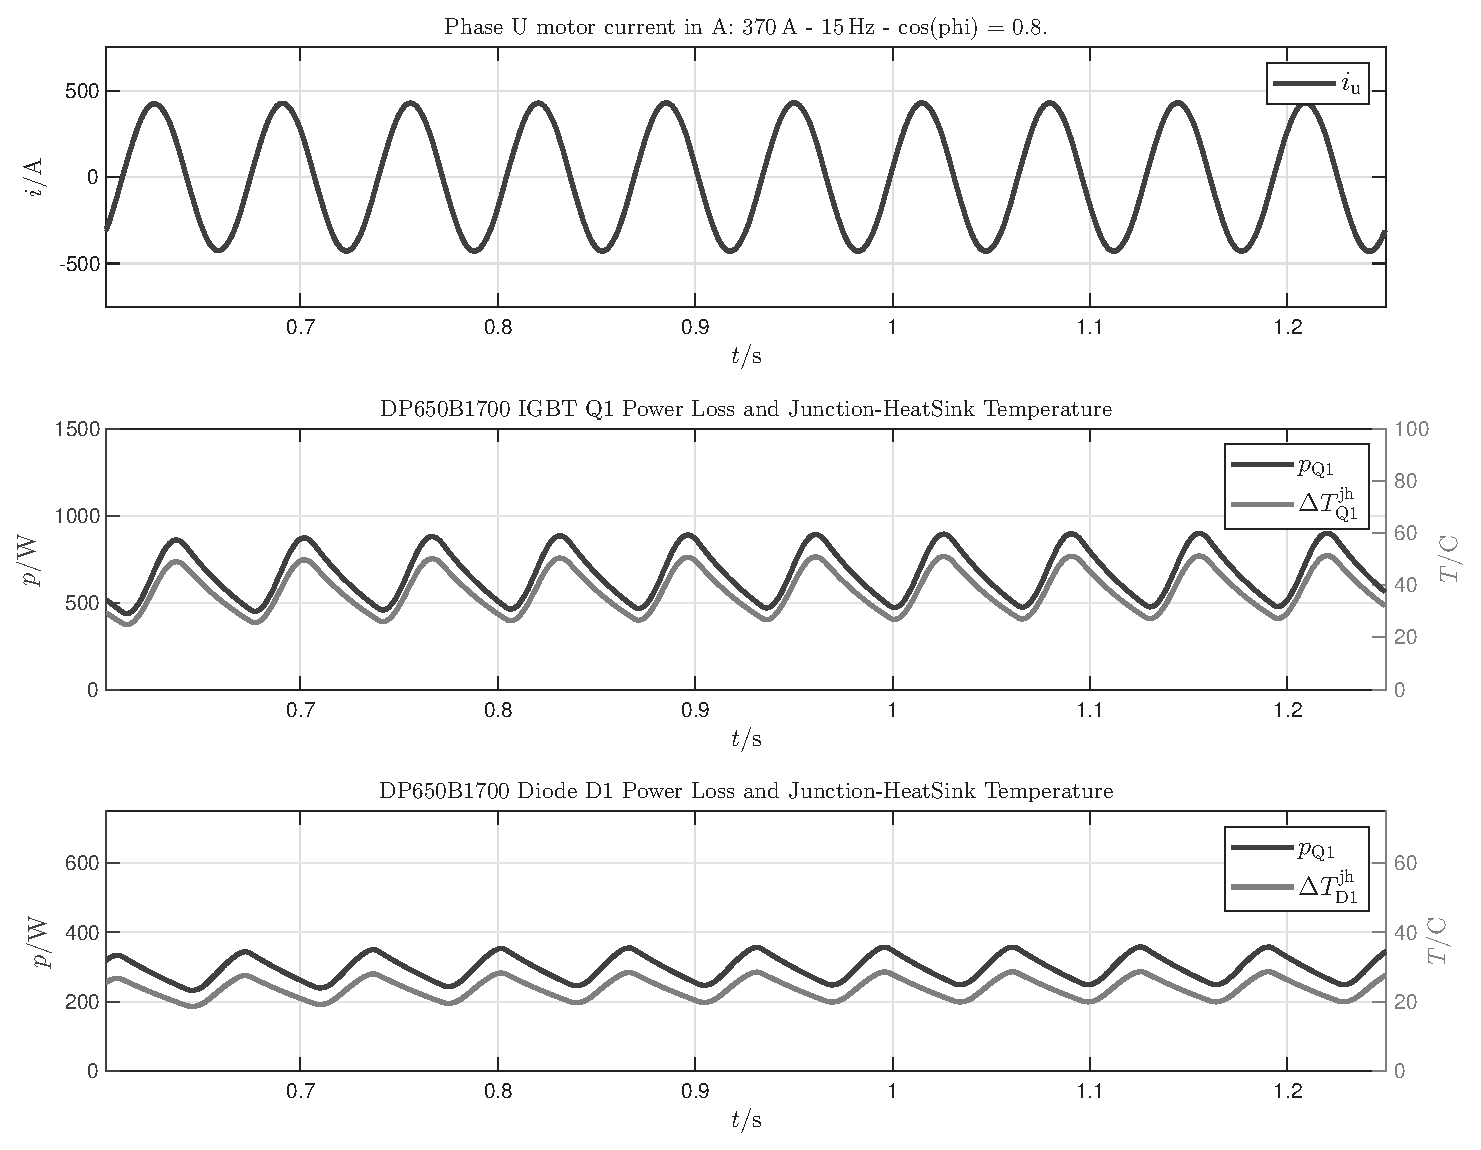
\includegraphics[width=225pt, angle=0,
			keepaspectratio]{figures/sim_results_DP650B1700_4kHz_370A_cosphi8p/thermal_behavior_Q1.eps}
			\captionsetup{width=0.65\textwidth, font=footnotesize}
			\caption{DP650B1700 Q1 IGBT thermal power/thermal behaviour at $I_\text{load}^\text{inv} = \SI{370}{\ampere}$.}
			\label{fig:sim_results_DP650B1700_4kHz_370A_cosphi8p}
		\end{subfigure}%
		\begin{subfigure}{0.5\textwidth}
			\centering
			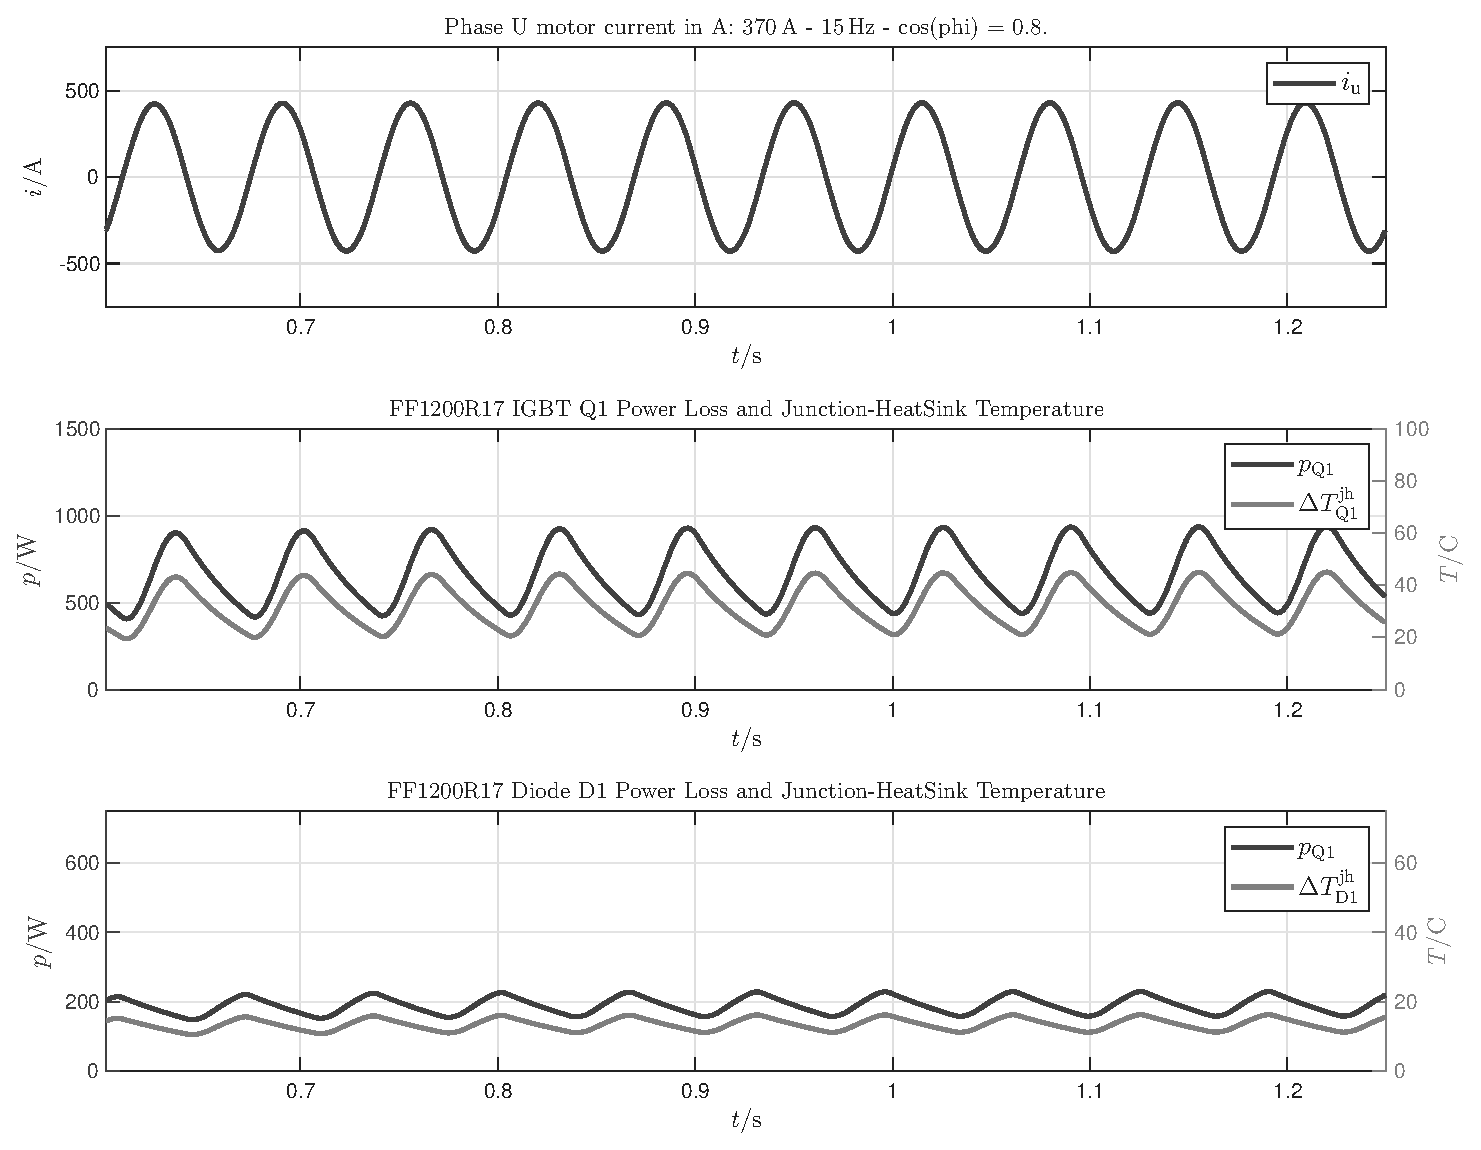
\includegraphics[width=225pt, angle=0,
			keepaspectratio]{figures/sim_results_FF1200R17_4kHz_370A_cosphi8p/thermal_behavior_Q1.eps}
			\captionsetup{width=0.65\textwidth, font=footnotesize}
			\caption{FF1200R17IP5P Q1 IGBT thermal power/thermal behaviour at $I_\text{load}^\text{inv} = \SI{370}{\ampere}$.}
			\label{fig:sim_results_FF1200R17_4kHz_370A_cosphi8p}
		\end{subfigure}
		\captionsetup{width=0.65\textwidth, font=small}
		\caption{Thermal behaviour comparison between IGBT DP650B1700 and FF1200R17IP5P at $I_\text{load}^\text{inv} = \SI{370}{\ampere}$.}
		\label{}
	\end{figure}
	
	\begin{itemize}
		\item[--] $I_\text{load}^\text{inv} = \SI{520}{\ampere}$, 140\% of the nominal inverter current;
		\item[--] $f_\text{pwm}^\text{inv} = \SI{4}{\kilo\hertz}$;
		\item[--] $T_\text{hs}^\text{inv} = \SI{65}{\celsius}$;
		\item[--] $\cos(\varphi) = 0.8$, driver mode;
		\item[--] $f_\text{load} = \SI{15}{\hertz}$, load frequency (critical parameter for maximum junction temperature evaluation);
		\item[--] driver board DB1.51 (new driver board).
	\end{itemize}
	\begin{figure}[H]
		\centering
		\begin{subfigure}{0.5\textwidth}
			\centering
			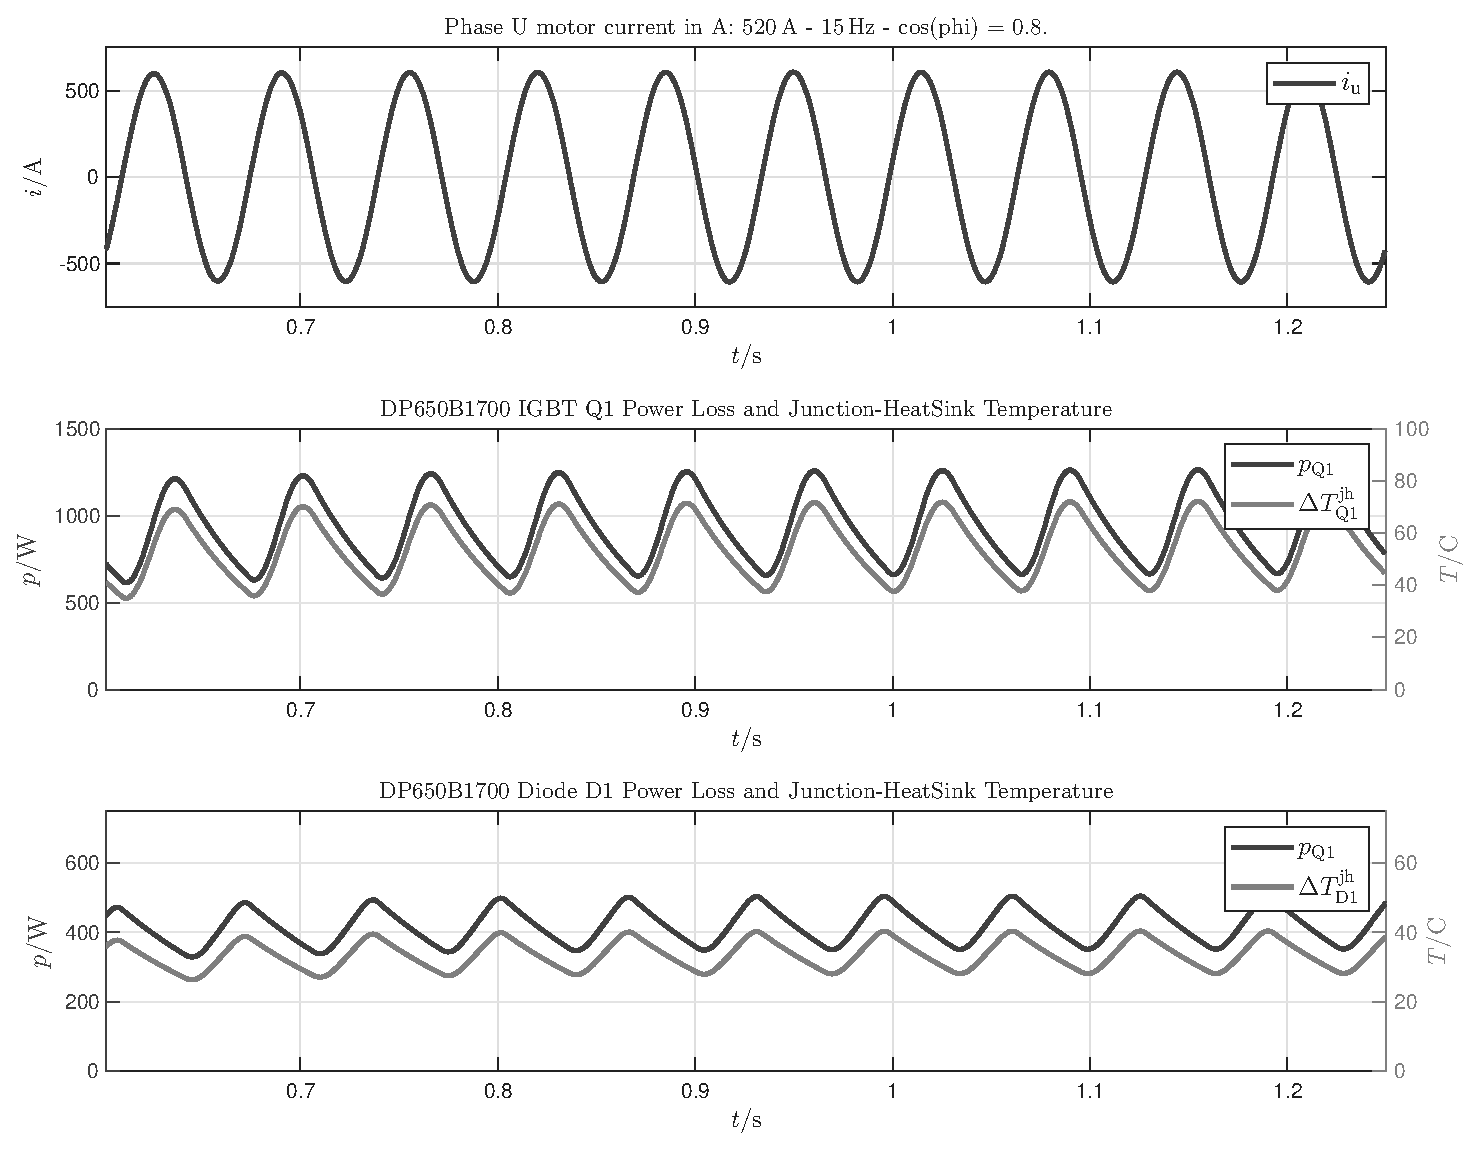
\includegraphics[width=225pt, angle=0,
			keepaspectratio]{figures/sim_results_DP650B1700_4kHz_520A_cosphi8p/thermal_behavior_Q1.eps}
			\captionsetup{width=0.65\textwidth, font=footnotesize}
			\caption{DP650B1700 Q1 IGBT thermal power/thermal behaviour at $I_\text{load}^\text{inv} = \SI{520}{\ampere}$.}
			\label{fig:sim_results_DP650B1700_4kHz_520A_cosphi8p}
		\end{subfigure}%
		\begin{subfigure}{0.5\textwidth}
			\centering
			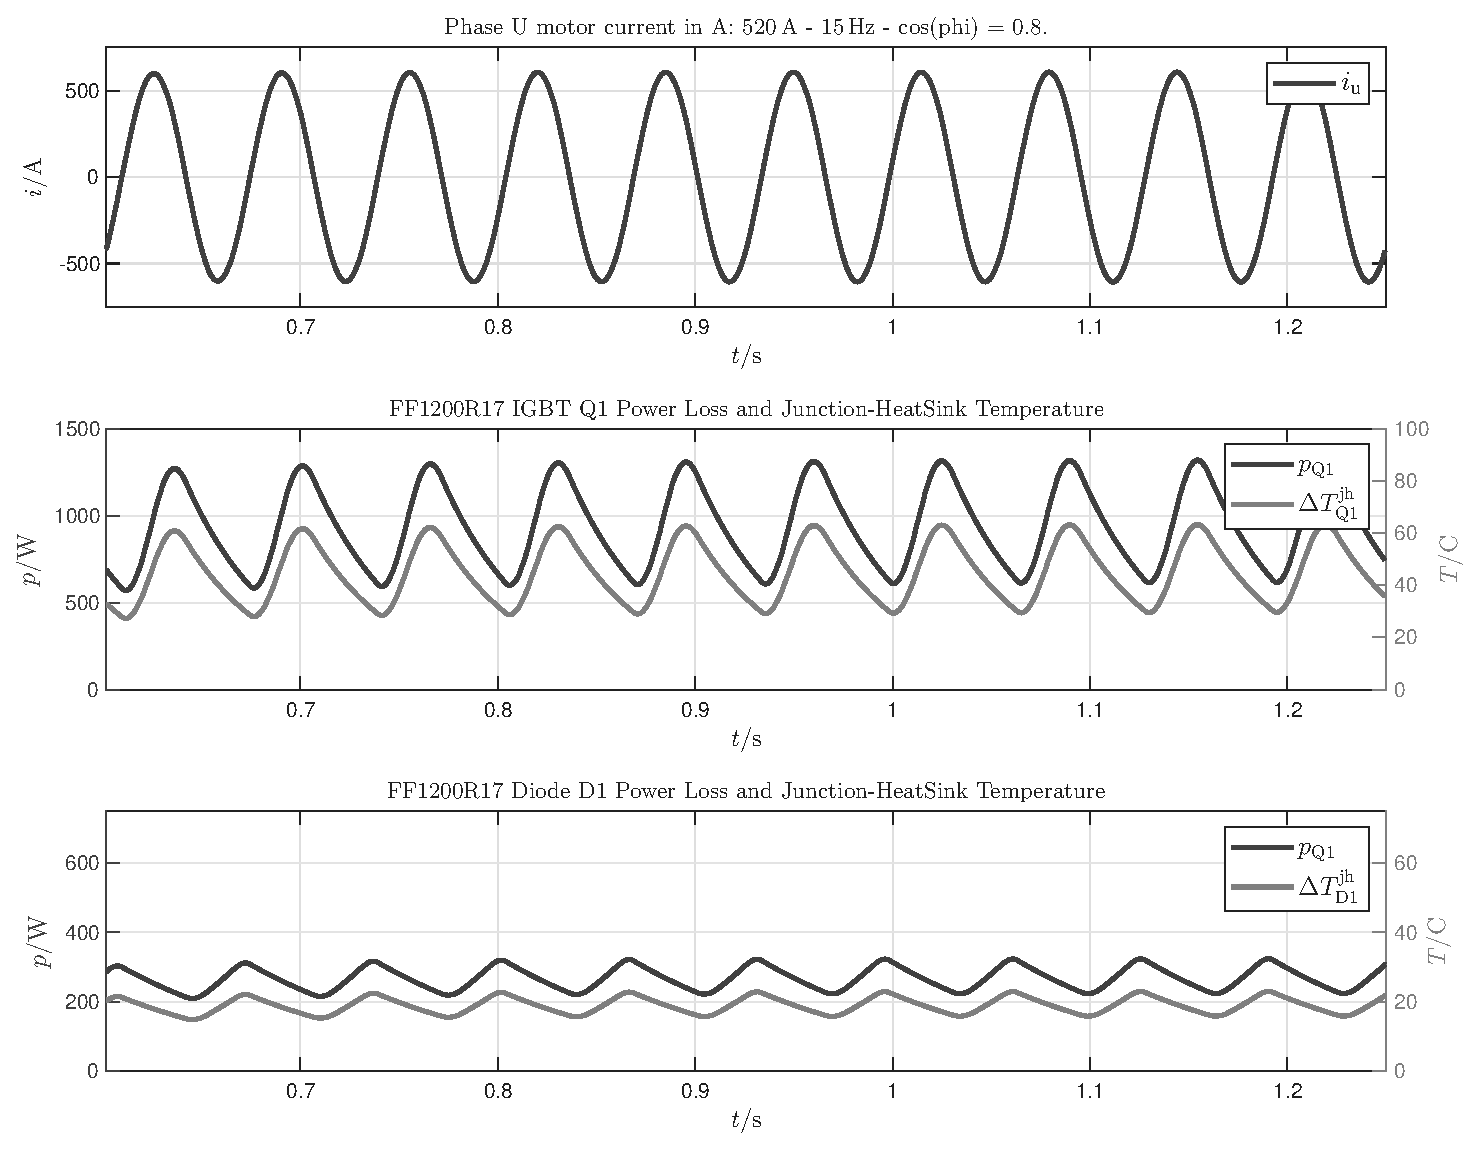
\includegraphics[width=225pt, angle=0,
			keepaspectratio]{figures/sim_results_FF1200R17_4kHz_520A_cosphi8p/thermal_behavior_Q1.eps}
			\captionsetup{width=0.65\textwidth, font=footnotesize}
			\caption{FF1200R17IP5P Q1 IGBT thermal power/thermal behaviour at $I_\text{load}^\text{inv} = \SI{520}{\ampere}$.}
			\label{fig:sim_results_FF1200R17_4kHz_520A_cosphi8p}
		\end{subfigure}
		\captionsetup{width=0.65\textwidth, font=small}
		\caption{Thermal behaviour comparison between IGBT DP650B1700 and FF1200R17IP5P at $I_\text{load}^\text{inv} = \SI{520}{\ampere}$.}
		\label{}
	\end{figure}

	\noindent Comparison between \textbf{FF650R17IE4} and \textbf{FF1200R17IP5P} under the same working condition.
	\begin{itemize}
		\item[--] $I_\text{load}^\text{inv} = \SI{370}{\ampere}$, 100\% of the nominal inverter current;
		\item[--] $f_\text{pwm}^\text{inv} = \SI{4}{\kilo\hertz}$;
		\item[--] $T_\text{hs}^\text{inv} = \SI{65}{\celsius}$;
		\item[--] $\cos(\varphi) = 0.8$, driver mode;
		\item[--] $f_\text{load} = \SI{15}{\hertz}$, load frequency (critical parameter for maximum junction temperature evaluation);
		\item[--] driver board DB1.51 (new driver board).
	\end{itemize}
	\begin{figure}[H]
		\centering
		\begin{subfigure}{0.5\textwidth}
			\centering
			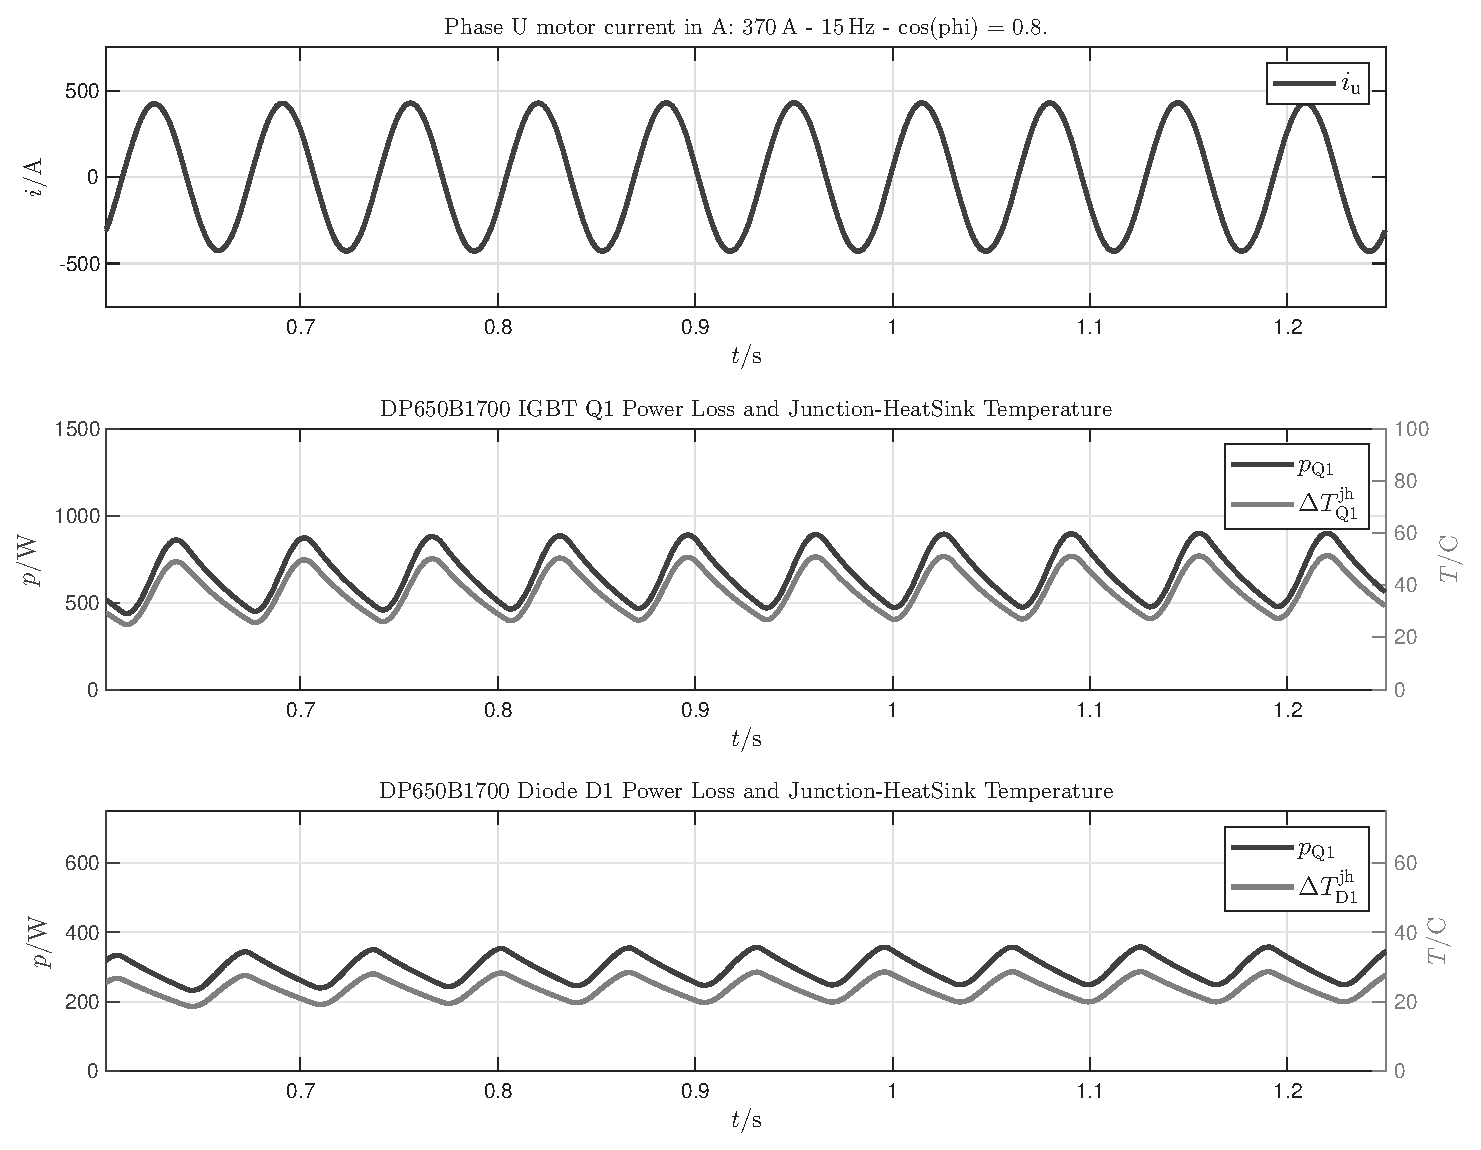
\includegraphics[width=225pt, angle=0,
			keepaspectratio]{figures/sim_results_DP650B1700_4kHz_370A_cosphi8p/thermal_behavior_Q1.eps}
			\captionsetup{width=0.65\textwidth, font=footnotesize}
			\caption{FF650R17IE4 Q1 IGBT thermal power/thermal behaviour at $I_\text{load}^\text{inv} = \SI{370}{\ampere}$.}
			\label{fig:sim_results_FF650R17IE4_4kHz_370A_cosphi8p}
		\end{subfigure}%
		\begin{subfigure}{0.5\textwidth}
			\centering
			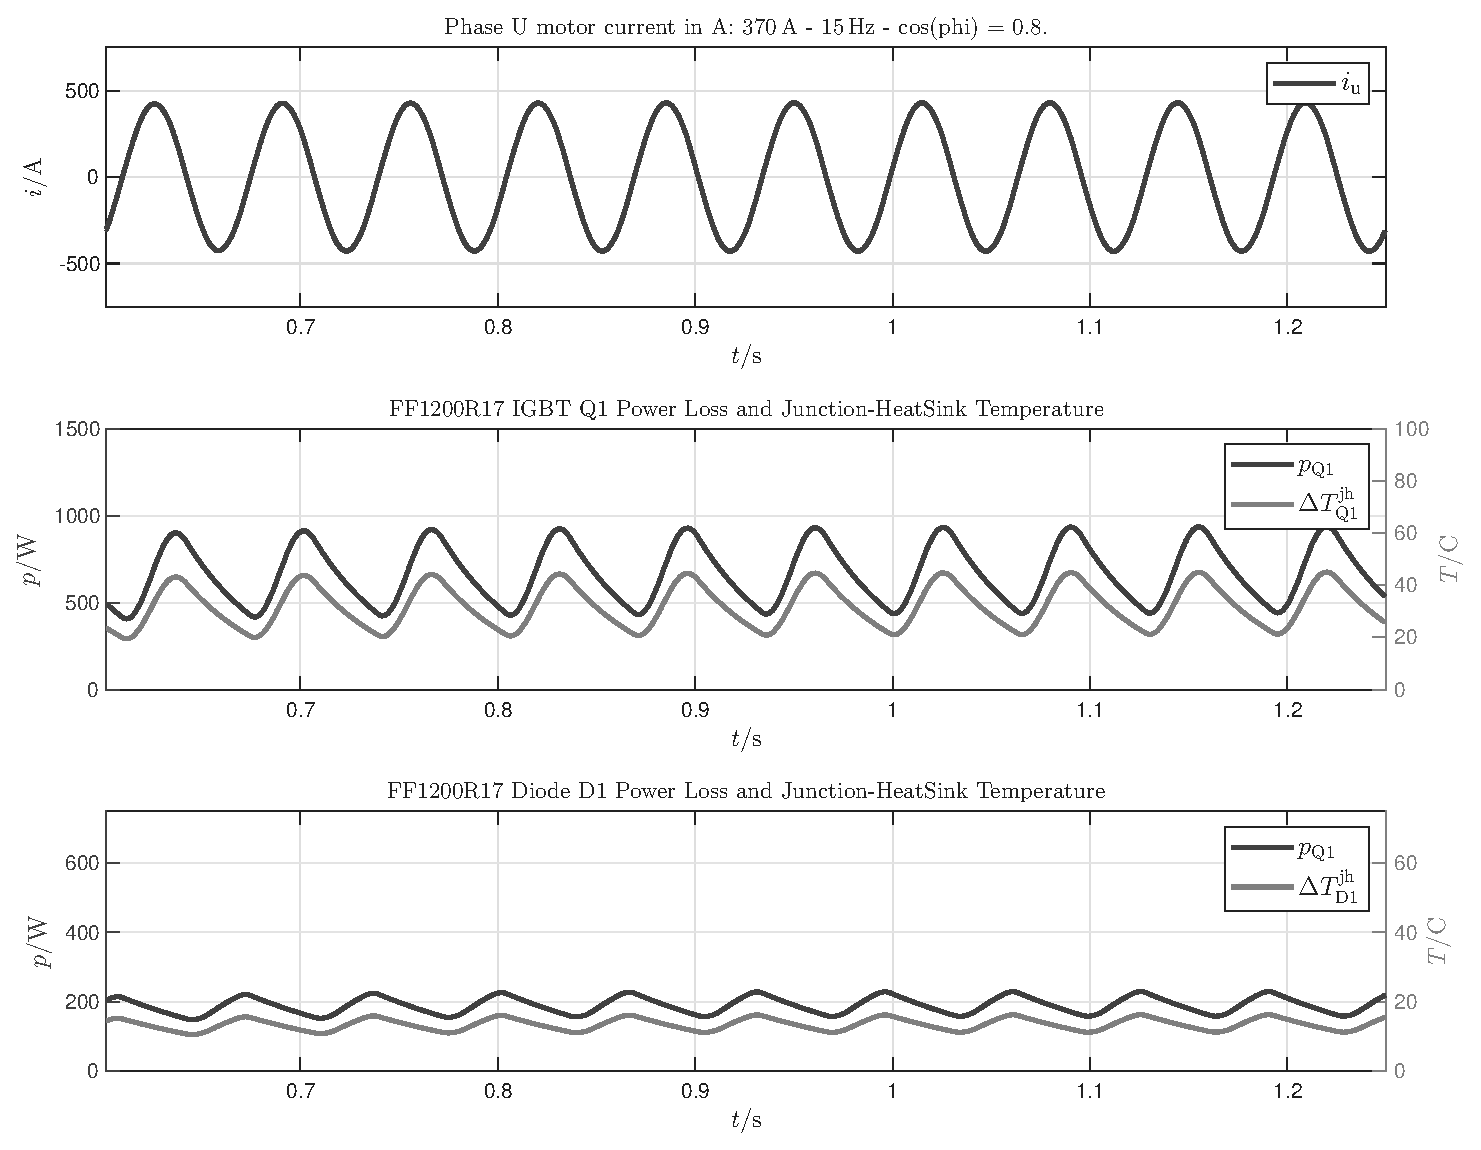
\includegraphics[width=225pt, angle=0,
			keepaspectratio]{figures/sim_results_FF1200R17_4kHz_370A_cosphi8p/thermal_behavior_Q1.eps}
			\captionsetup{width=0.65\textwidth, font=footnotesize}
			\caption{FF1200R17IP5P Q1 IGBT thermal power/thermal behaviour at $I_\text{load}^\text{inv} = \SI{370}{\ampere}$.}
			\label{}
		\end{subfigure}
		\captionsetup{width=0.65\textwidth, font=small}
		\caption{Thermal behaviour comparison between IGBT FF650R17IE4 and FF1200R17IP5P at $I_\text{load}^\text{inv} = \SI{370}{\ampere}$.}
		\label{}
	\end{figure}
	
	\begin{itemize}
		\item[--] $I_\text{load}^\text{inv} = \SI{520}{\ampere}$, 140\% of the nominal inverter current;
		\item[--] $f_\text{pwm}^\text{inv} = \SI{4}{\kilo\hertz}$;
		\item[--] $T_\text{hs}^\text{inv} = \SI{65}{\celsius}$;
		\item[--] $\cos(\varphi) = 0.8$, driver mode;
		\item[--] $f_\text{load} = \SI{15}{\hertz}$, load frequency (critical parameter for maximum junction temperature evaluation);
		\item[--] driver board DB1.51 (new driver board).
	\end{itemize}
	\begin{figure}[H]
		\centering
		\begin{subfigure}{0.5\textwidth}
			\centering
			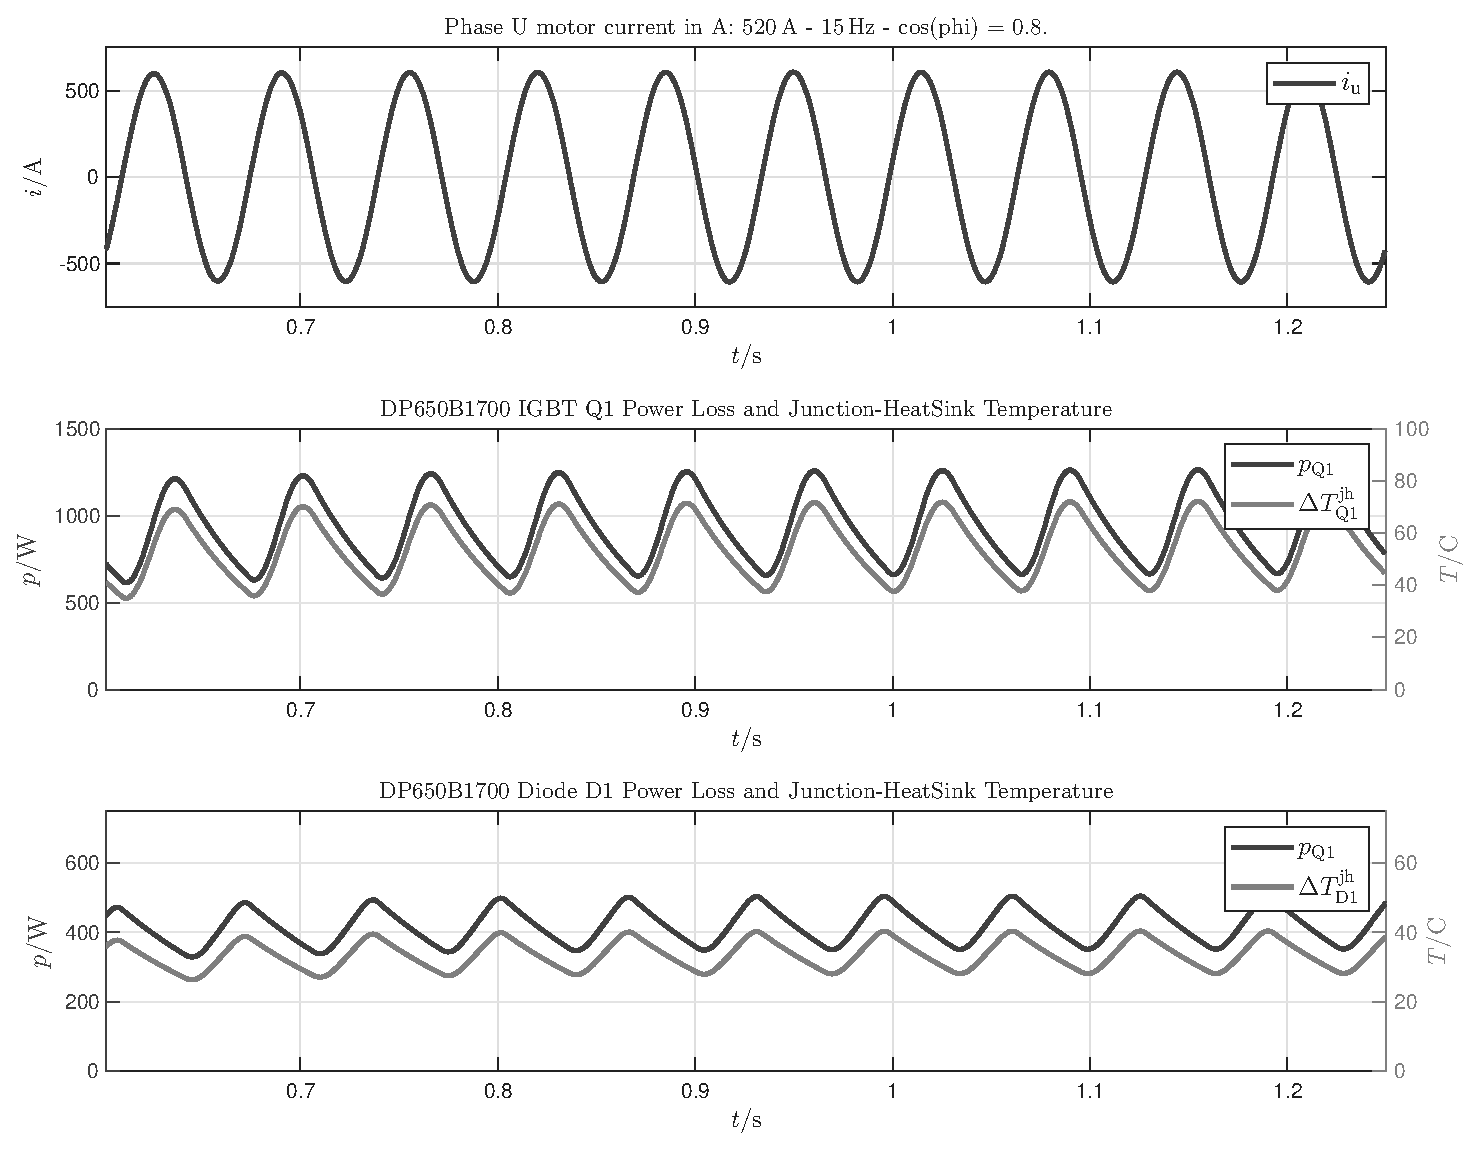
\includegraphics[width=225pt, angle=0,
			keepaspectratio]{figures/sim_results_DP650B1700_4kHz_520A_cosphi8p/thermal_behavior_Q1.eps}
			\captionsetup{width=0.65\textwidth, font=footnotesize}
			\caption{FF650R17IE4 Q1 IGBT thermal power/thermal behaviour at $I_\text{load}^\text{inv} = \SI{520}{\ampere}$.}
			\label{fig:sim_results_FF650R17IE4_4kHz_520A_cosphi8p}
		\end{subfigure}%
		\begin{subfigure}{0.5\textwidth}
			\centering
			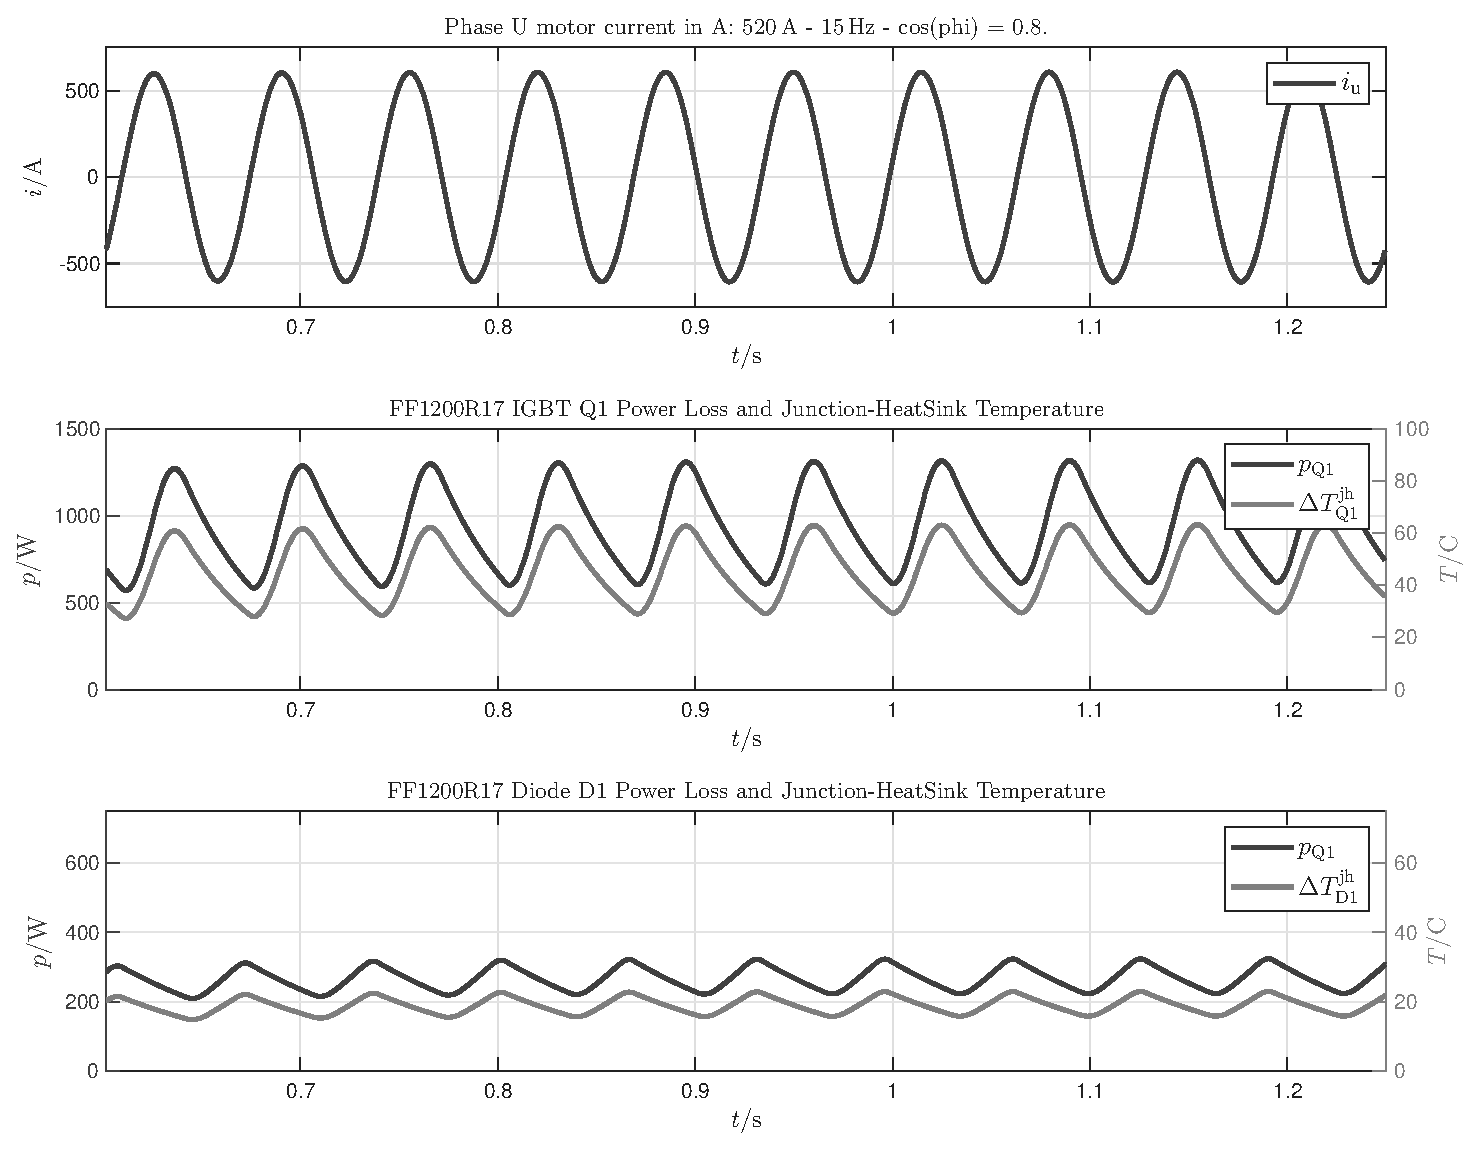
\includegraphics[width=225pt, angle=0,
			keepaspectratio]{figures/sim_results_FF1200R17_4kHz_520A_cosphi8p/thermal_behavior_Q1.eps}
			\captionsetup{width=0.65\textwidth, font=footnotesize}
			\caption{FF1200R17IP5P Q1 IGBT thermal power/thermal behaviour at $I_\text{load}^\text{inv} = \SI{520}{\ampere}$.}
			\label{}
		\end{subfigure}
		\captionsetup{width=0.65\textwidth, font=small}
		\caption{Thermal behaviour comparison between IGBT FF650R17IE4 and FF1200R17IP5P at $I_\text{load}^\text{inv} = \SI{520}{\ampere}$.}
		\label{}
	\end{figure}

	\subsubsection{Simulation results in tables}
	
	\noindent\textbf{Simulation results case scenario 1}
	\begin{itemize}
		\item[--] $I_\text{load}^\text{inv} = \SI{370}{\ampere}$, 100\% of the nominal inverter current;
		\item[--] $f_\text{pwm}^\text{inv} = \SI{4}{\kilo\hertz}$;
		\item[--] $T_\text{hs}^\text{inv} = \SI{65}{\celsius}$;
		\item[--] $\cos(\varphi) = 0.8$, drive mode;
		\item[--] $f_\text{load} = \SI{15}{\hertz}$, load frequency (critical parameter for maximum junction temperature evaluation);
	\end{itemize}
	
	\newcolumntype{W}{>{\hsize=2\hsize}X}
	\newcolumntype{H}{>{\centering\arraybackslash\hsize=0.8\hsize}X}
	
	\begin{table}[H]
		\centering
		\captionsetup{width=0.75\textwidth, font=small}
		\caption{\textbf{Simulation results case scenario 1} --- Power losses and maximum junction temperature at $I_\text{load}^\text{inv} = \SI{370}{\ampere}$, $f_\text{pwm}^\text{inv} = \SI{4}{\kilo\hertz}$, $T_\text{hs}^\text{inv} = \SI{65}{\celsius}$, $\cos(\varphi) = 0.8$.}
		\label{}
		\renewcommand{\arraystretch}{2.0}
		\begin{tabularx}{\textwidth}{W|H|H|H|H|H}
			\hline\hline
			& $T_\text{j}^\text{Q}$ & $T_\text{j}^\text{D}$ & $P_\text{Q}$ & $P_\text{D}$ & $\Delta T_\text{j}$ \\
			\hline
			FF650R17IE4 & \SI{120}{\celsius} & \SI{70}{\celsius}  & \SI{760}{\watt} & \SI{200}{\watt}  & \SI{30}{\celsius} \\
			\hline
			D650B1700 & \SI{112}{\celsius} & \SI{74}{\celsius}  & \SI{666}{\watt} & \SI{297}{\watt}  & \SI{26}{\celsius} \\
			\hline
			FF1200R17IP5P  & \SI{106}{\celsius} & \SI{61}{\celsius}  & \SI{665}{\watt} & \SI{189}{\watt}  & \SI{17}{\celsius} \\
			\hline\hline
		\end{tabularx}
	\end{table}
	
	\vspace{5mm}
	\noindent\textbf{Simulation results case scenario 2}
	\begin{itemize}
		\item[--] $I_\text{load}^\text{inv} = \SI{520}{\ampere}$, 140\% of the nominal inverter current;
		\item[--] $f_\text{pwm}^\text{inv} = \SI{4}{\kilo\hertz}$;
		\item[--] $T_\text{hs}^\text{inv} = \SI{65}{\celsius}$;
		\item[--] $\cos(\varphi) = 0.8$, drive mode;
		\item[--] $f_\text{load} = \SI{15}{\hertz}$, load frequency (critical parameter for maximum junction temperature evaluation);
	\end{itemize}
	\begin{table}[H]
		\centering
		\captionsetup{width=0.75\textwidth, font=small}
		\caption{\textbf{Simulation results case scenario 2} --- Power losses and maximum junction temperature at $I_\text{load}^\text{inv} = \SI{520}{\ampere}$, $f_\text{pwm}^\text{inv} = \SI{4}{\kilo\hertz}$, $T_\text{hs}^\text{inv} = \SI{65}{\celsius}$, $\cos(\varphi) = 0.8$}
		\label{}
		\renewcommand{\arraystretch}{2.0}
		\begin{tabularx}{\textwidth}{W|H|H|H|H|H}
			\hline\hline
			& $T_\text{j}^\text{Q}$ & $T_\text{j}^\text{D}$ & $P_\text{Q}$ & $P_\text{D}$ & $\Delta T_\text{j}$ \\
			\hline
			FF650R17IE4    & \SI{152}{\celsius} & \SI{82}{\celsius}  & \SI{1066}{\watt} & \SI{276}{\watt}  & \SI{42}{\celsius} \\
			\hline
			FF650R17IE4DB2 & \SI{141}{\celsius} & \SI{88}{\celsius}  & \SI{940}{\watt} & \SI{417}{\watt}  & \SI{37}{\celsius} \\
			\hline
			FF1200R17IP5P  & \SI{132}{\celsius} & \SI{70}{\celsius}  & \SI{937}{\watt} & \SI{266}{\watt}  & \SI{23}{\celsius} \\
			\hline\hline
		\end{tabularx}
	\end{table}
	
	\section{Double pulse tests}
	\label{sec:scope}
	This section presents the results of Double Pulse Tests (DPTs) conducted
	to assess the performance of the FF1200R17IP5P IGBT module in conjunction with
	the new driver board DB1.51.
	The following test configurations were evaluated:
	\begin{itemize}
		\item[--] \textbf{DPT\,1}: DP650B1700 with DB1.00;
		\begin{itemize}
			\item[--] series-production IGBT module with series-production driver board;
		\end{itemize}
		\item[--] \textbf{DPT\,2}: DP650B1700 with DB1.51;
		\begin{itemize}
			\item[--] series-production IGBT module with candidate driver board;
		\end{itemize}
		\item[--] \textbf{DPT\,3}: FF1200R17IP5P with DB1.00;
		\begin{itemize}
			\item[--] candidate IGBT module with series-production driver board;
		\end{itemize}
		\item[--] \textbf{DPT\,4}: FF1200R17IP5P with DB1.51;
		\begin{itemize}
			\item[--] candidate IGBT module with candidate driver board.
		\end{itemize}
	\end{itemize}


		\section{Measurement Results}
		\subsection{Turn-OFF}
		The following waveform were acquired at the first turn-off command.\\
		
		\noindent\textbf{Remark}: DB1.00 mounts higher turn-off resistors ($R_\text{g}^\text{off}$) than DB1.51, but DB1.51 implements a gate-emitter voltage rate limiter which led IGBTs to a lower turn-off collector-emitter overshoot ($\Delta u_\text{ce}$), as depicted in Figure~\ref{fig:turn_off_DP650_DB100_DB151}.\\
		
		
		
		\begin{figure}[H]
			\centering
			\begin{subfigure}{0.5\textwidth}
				\centering
				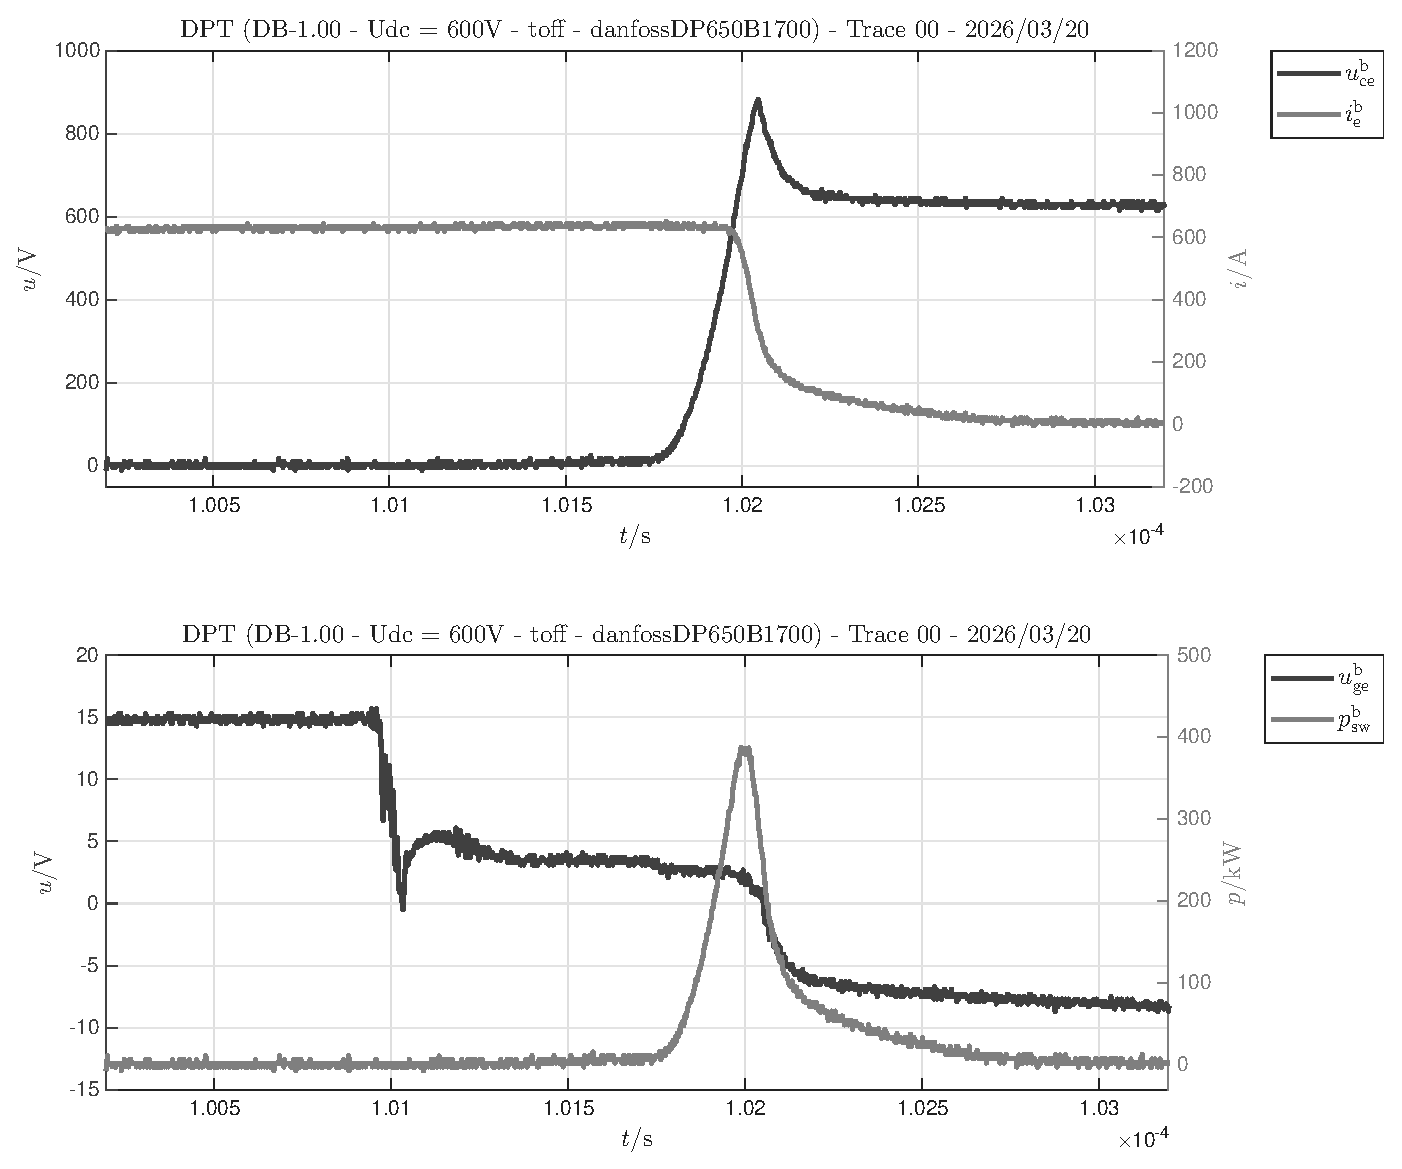
\includegraphics[width=225pt, angle=0,
				keepaspectratio]{figures/dpts/dpt_turn_off_udc600V_DP650_DB100.eps}
				\captionsetup{width=0.65\textwidth, font=footnotesize}
				\caption{Turn-OFF: DP650B1700 with DB1.00.}
				\label{fig:turn_off_DP650_DB100}
			\end{subfigure}%
			\begin{subfigure}{0.5\textwidth}
				\centering
				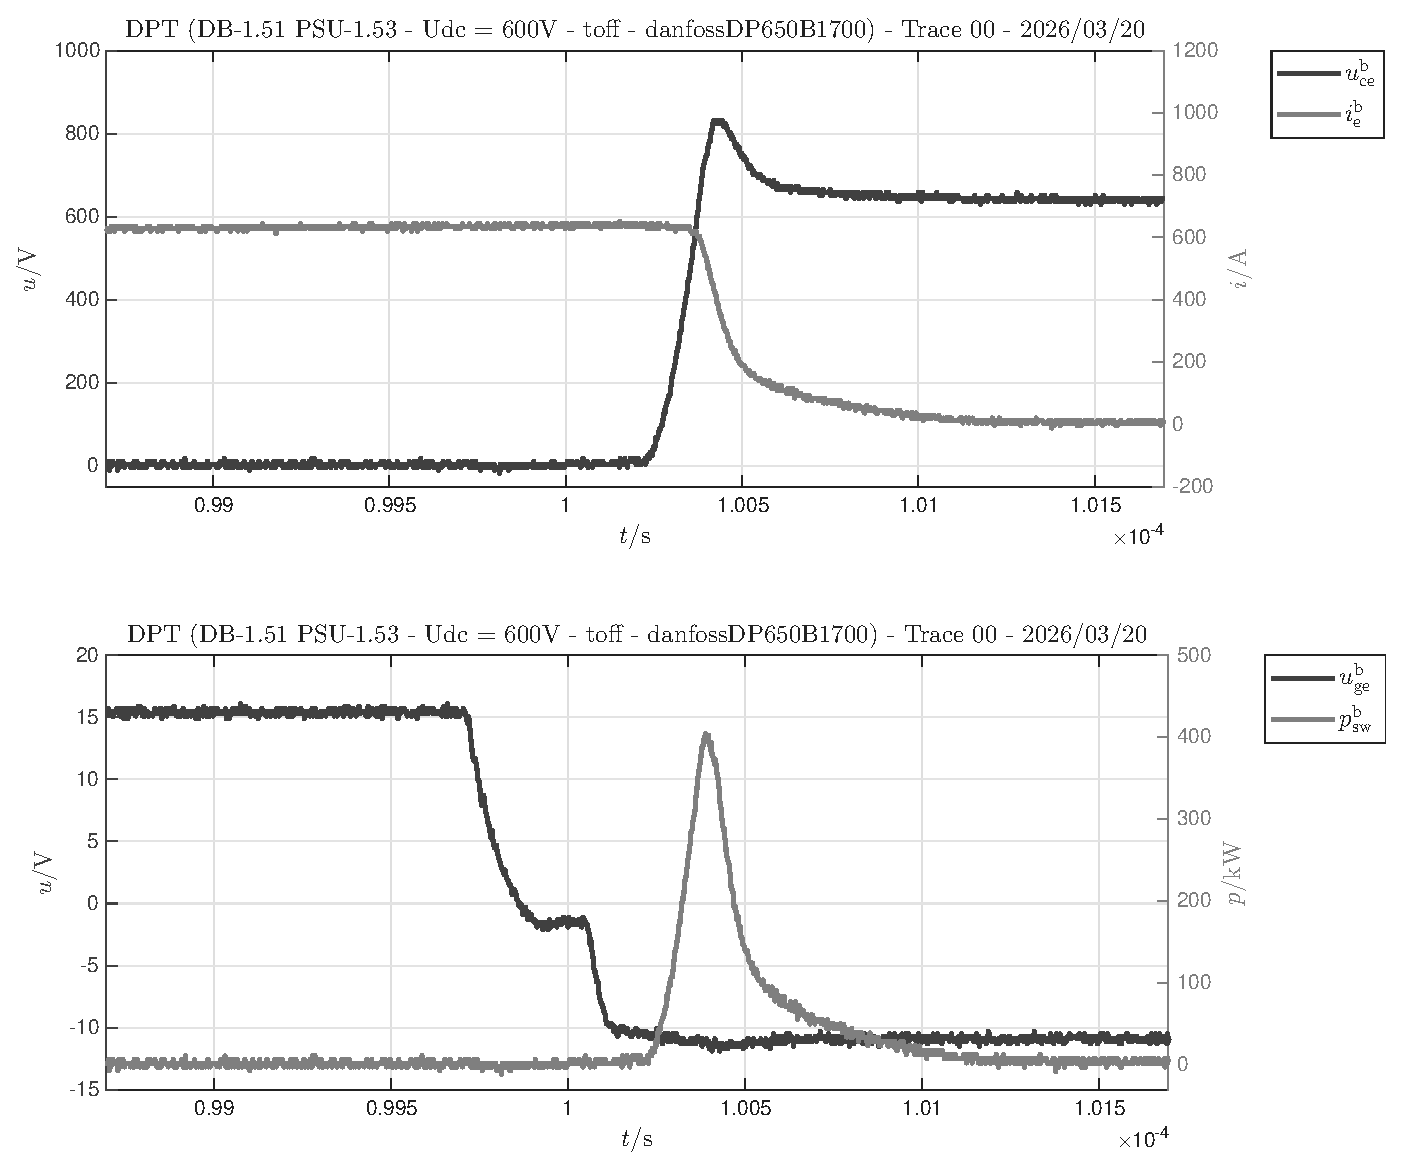
\includegraphics[width=225pt, angle=0,
				keepaspectratio]{figures/dpts/dpt_turn_off_udc600V_DP650_DB151.eps}
				\captionsetup{width=0.65\textwidth, font=footnotesize}
				\caption{Turn-OFF: DP650B1700 with DB1.51.}
				\label{fig:turn_off_DP650_DB151}
			\end{subfigure}
			\captionsetup{width=0.65\textwidth, font=small}
			\caption{Turn-OFF comparison: DP650B1700 with DB1.00 and DB1.51.}
			\label{fig:turn_off_DP650_DB100_DB151}
		\end{figure}

		\begin{figure}[H]
			\centering
			\begin{subfigure}{0.5\textwidth}
				\centering
				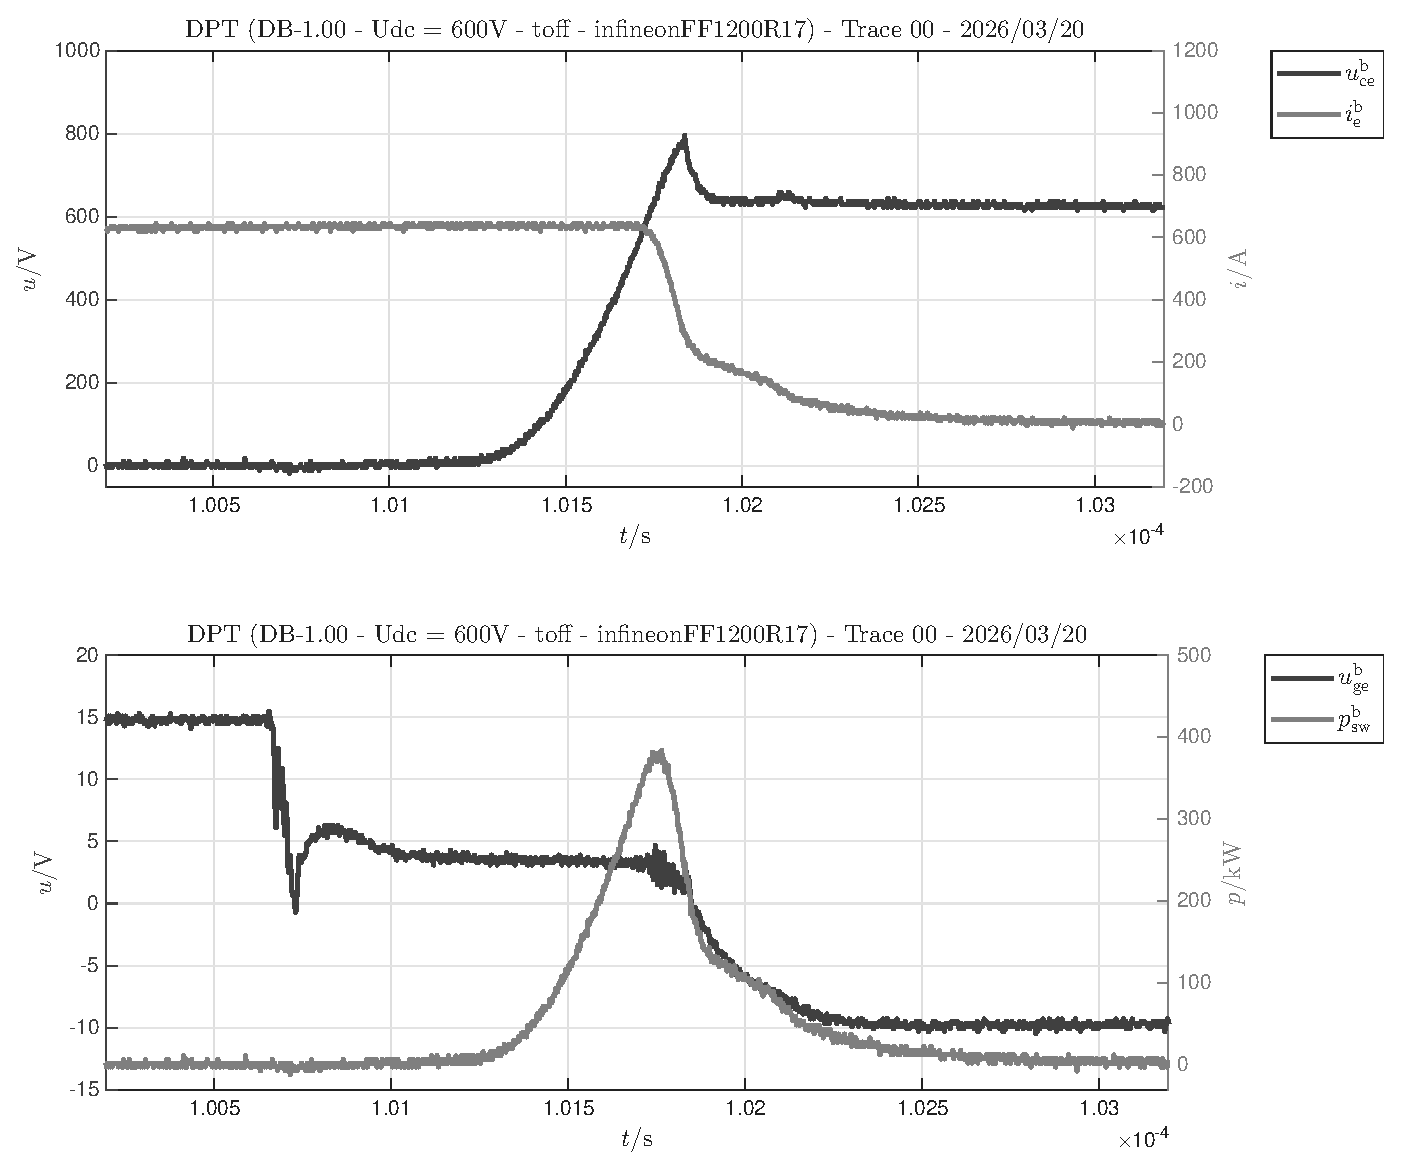
\includegraphics[width=225pt, angle=0,
				keepaspectratio]{figures/dpts/dpt_turn_off_udc600V_FF1200_DB100.eps}
				\captionsetup{width=0.65\textwidth, font=footnotesize}
				\caption{Turn-OFF: FF1200R17IP5P with DB1.00.}
				\label{fig:turn_off_FF1200_DB100}
			\end{subfigure}%
			\begin{subfigure}{0.5\textwidth}
				\centering
				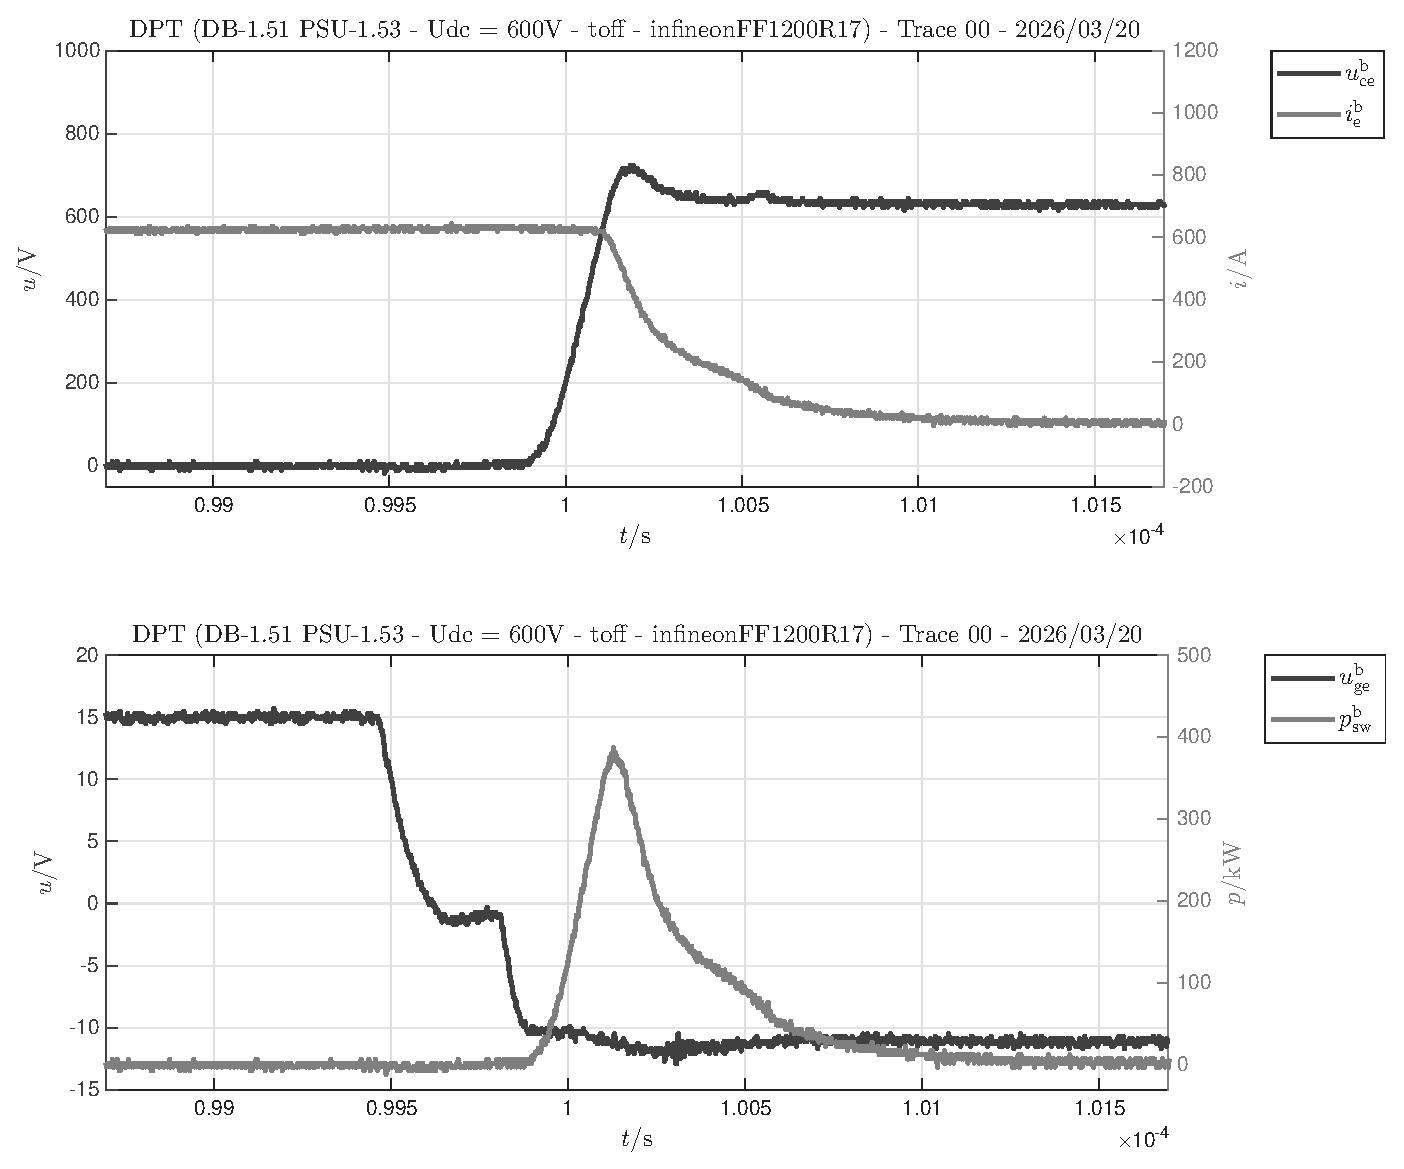
\includegraphics[width=225pt, angle=0,
				keepaspectratio]{figures/dpts/dpt_turn_off_udc600V_FF1200_DB151.eps}
				\captionsetup{width=0.65\textwidth, font=footnotesize}
				\caption{Turn-OFF: FF1200R17IP5P with DB1.51.}
				\label{fig:turn_off_FF1200_DB151}
			\end{subfigure}
			\captionsetup{width=0.65\textwidth, font=small}
			\caption{Turn-OFF comparison: FF1200R17IP5P with DB1.00 and DB1.51.}
			\label{fig:turn_off_FF1200_DB100_DB151}
		\end{figure}

		\begin{figure}[H]
			\centering
			\begin{subfigure}{0.5\textwidth}
				\centering
				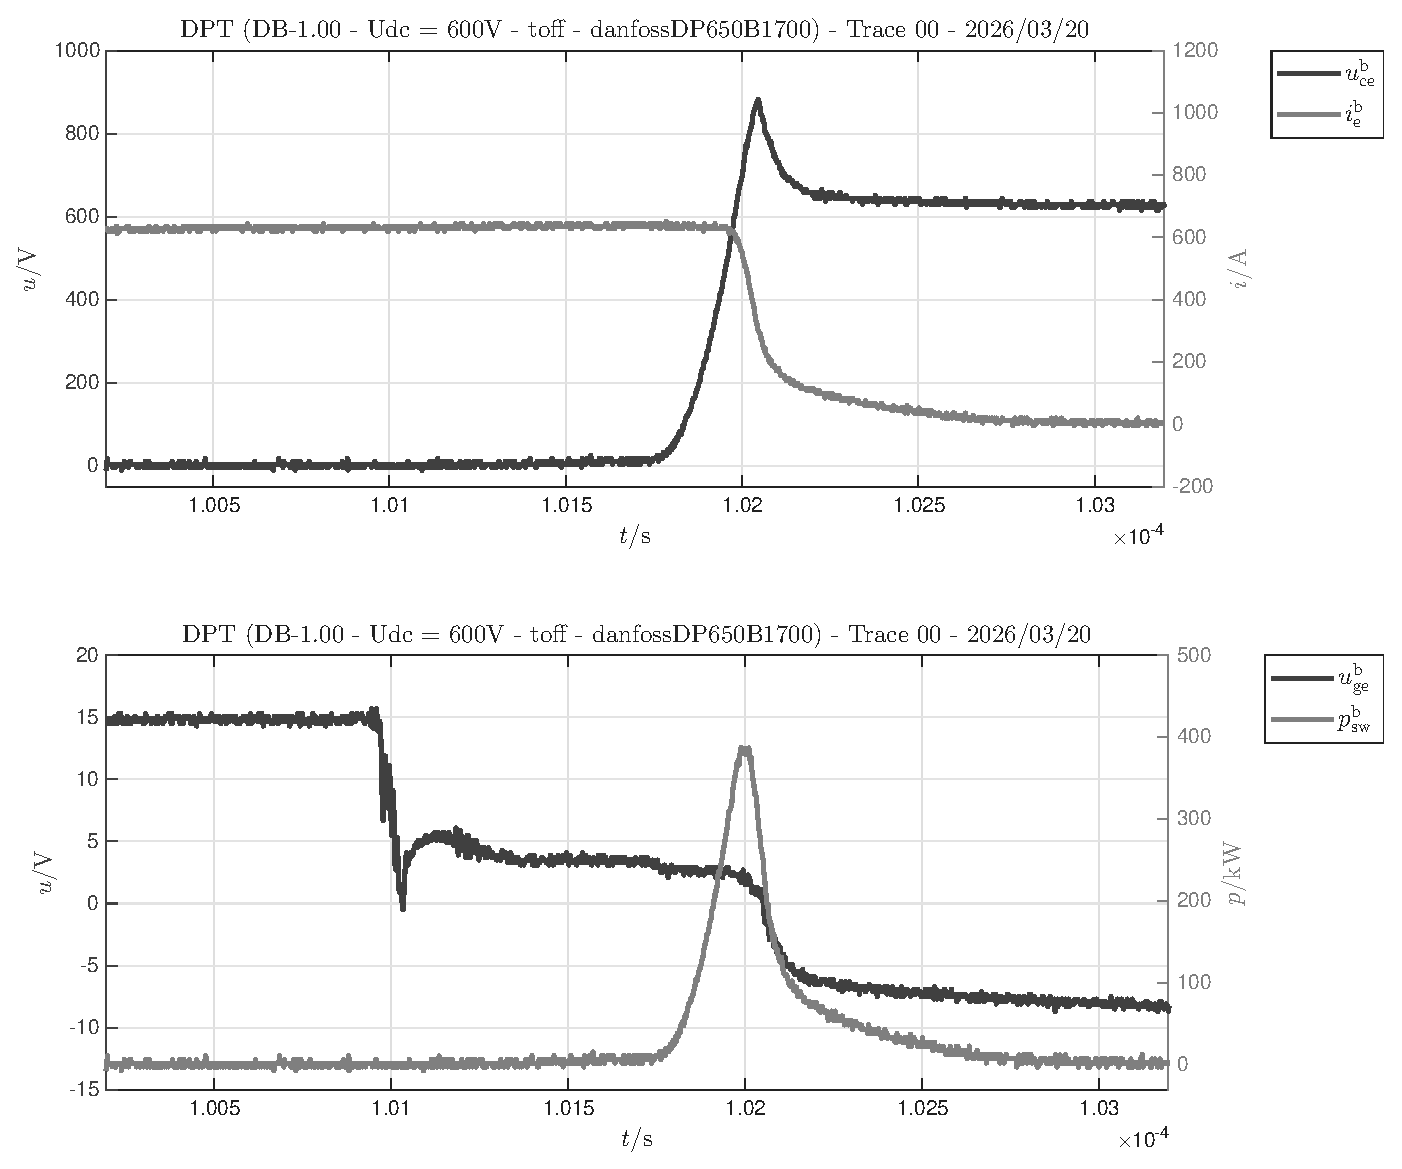
\includegraphics[width=225pt, angle=0,
				keepaspectratio]{figures/dpts/dpt_turn_off_udc600V_DP650_DB100.eps}
				\captionsetup{width=0.65\textwidth, font=footnotesize}
				\caption{Turn-OFF: DP650B1700 with DB1.00.}
				\label{fig:turn_off_DP650_DB100_b}
			\end{subfigure}%
			\begin{subfigure}{0.5\textwidth}
				\centering
				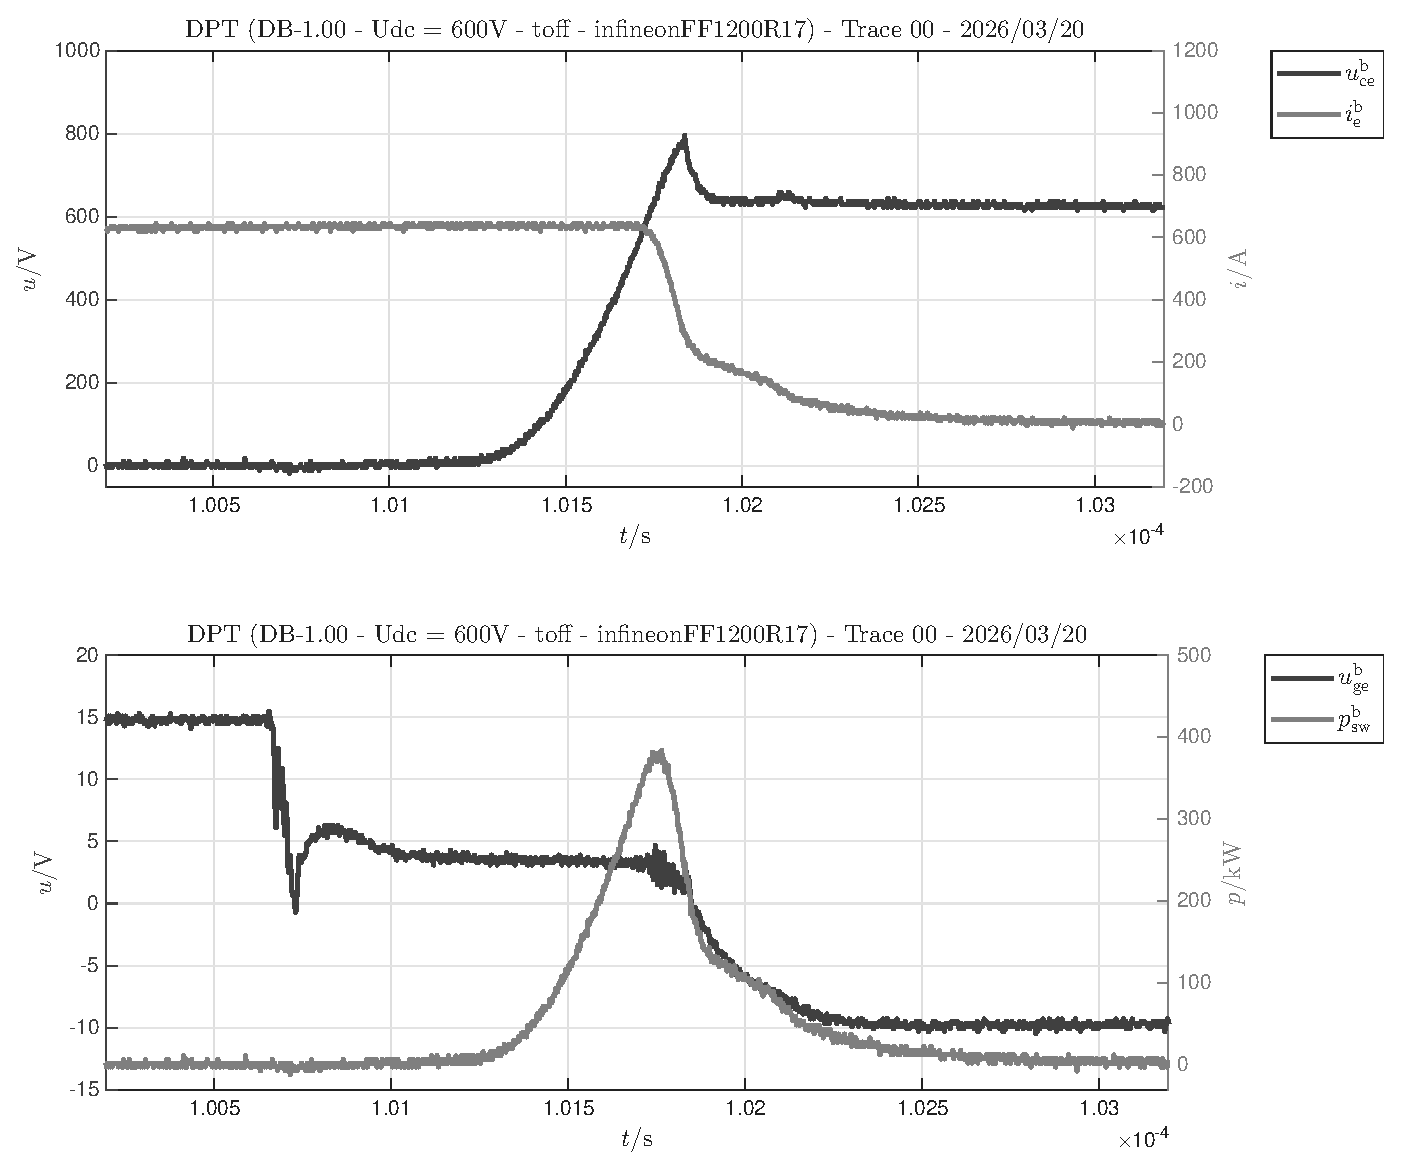
\includegraphics[width=225pt, angle=0,
				keepaspectratio]{figures/dpts/dpt_turn_off_udc600V_FF1200_DB100.eps}
				\captionsetup{width=0.65\textwidth, font=footnotesize}
				\caption{Turn-OFF: FF1200R17IP5P with DB1.00.}
				\label{fig:turn_off_FF1200_DB100_b}
			\end{subfigure}
			\captionsetup{width=0.65\textwidth, font=small}
			\caption{Turn-OFF comparison: DP650B1700 and FF1200R17IP5P with DB1.00.}
			\label{fig:turn_off_DP650_FF1200_DB100}
		\end{figure}

		\begin{figure}[H]
			\centering
			\begin{subfigure}{0.5\textwidth}
				\centering
				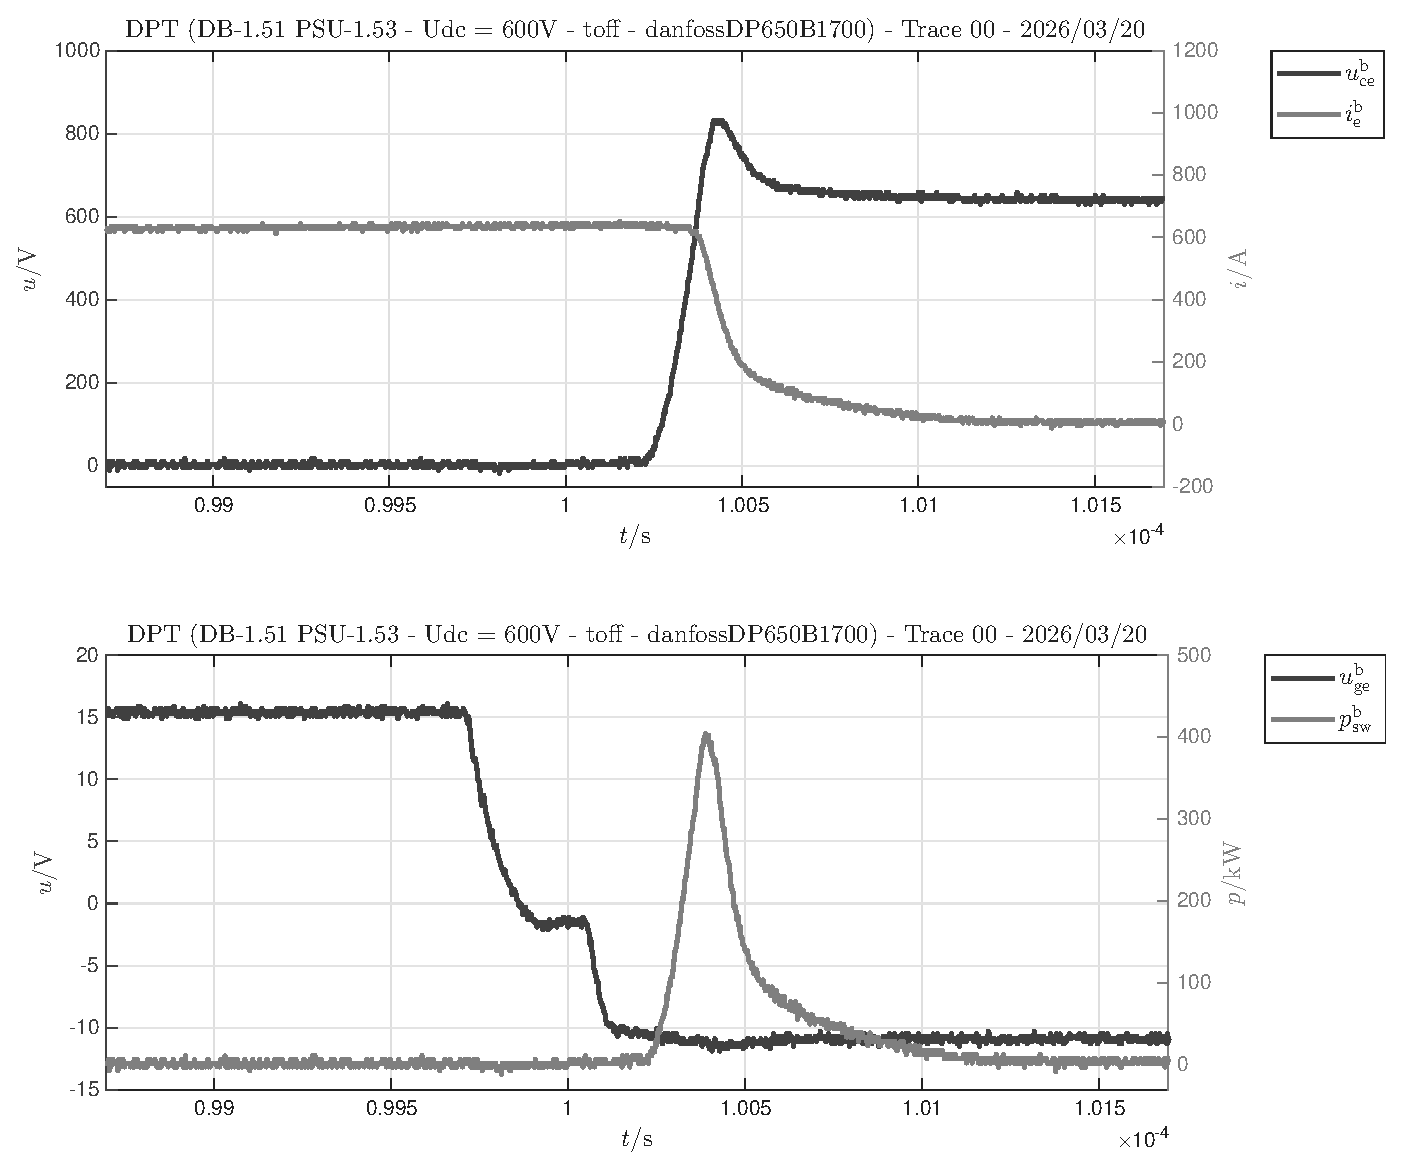
\includegraphics[width=225pt, angle=0,
				keepaspectratio]{figures/dpts/dpt_turn_off_udc600V_DP650_DB151.eps}
				\captionsetup{width=0.65\textwidth, font=footnotesize}
				\caption{Turn-OFF: DP650B1700 with DB1.51.}
				\label{fig:turn_off_DP650_DB151_b}
			\end{subfigure}%
			\begin{subfigure}{0.5\textwidth}
				\centering
				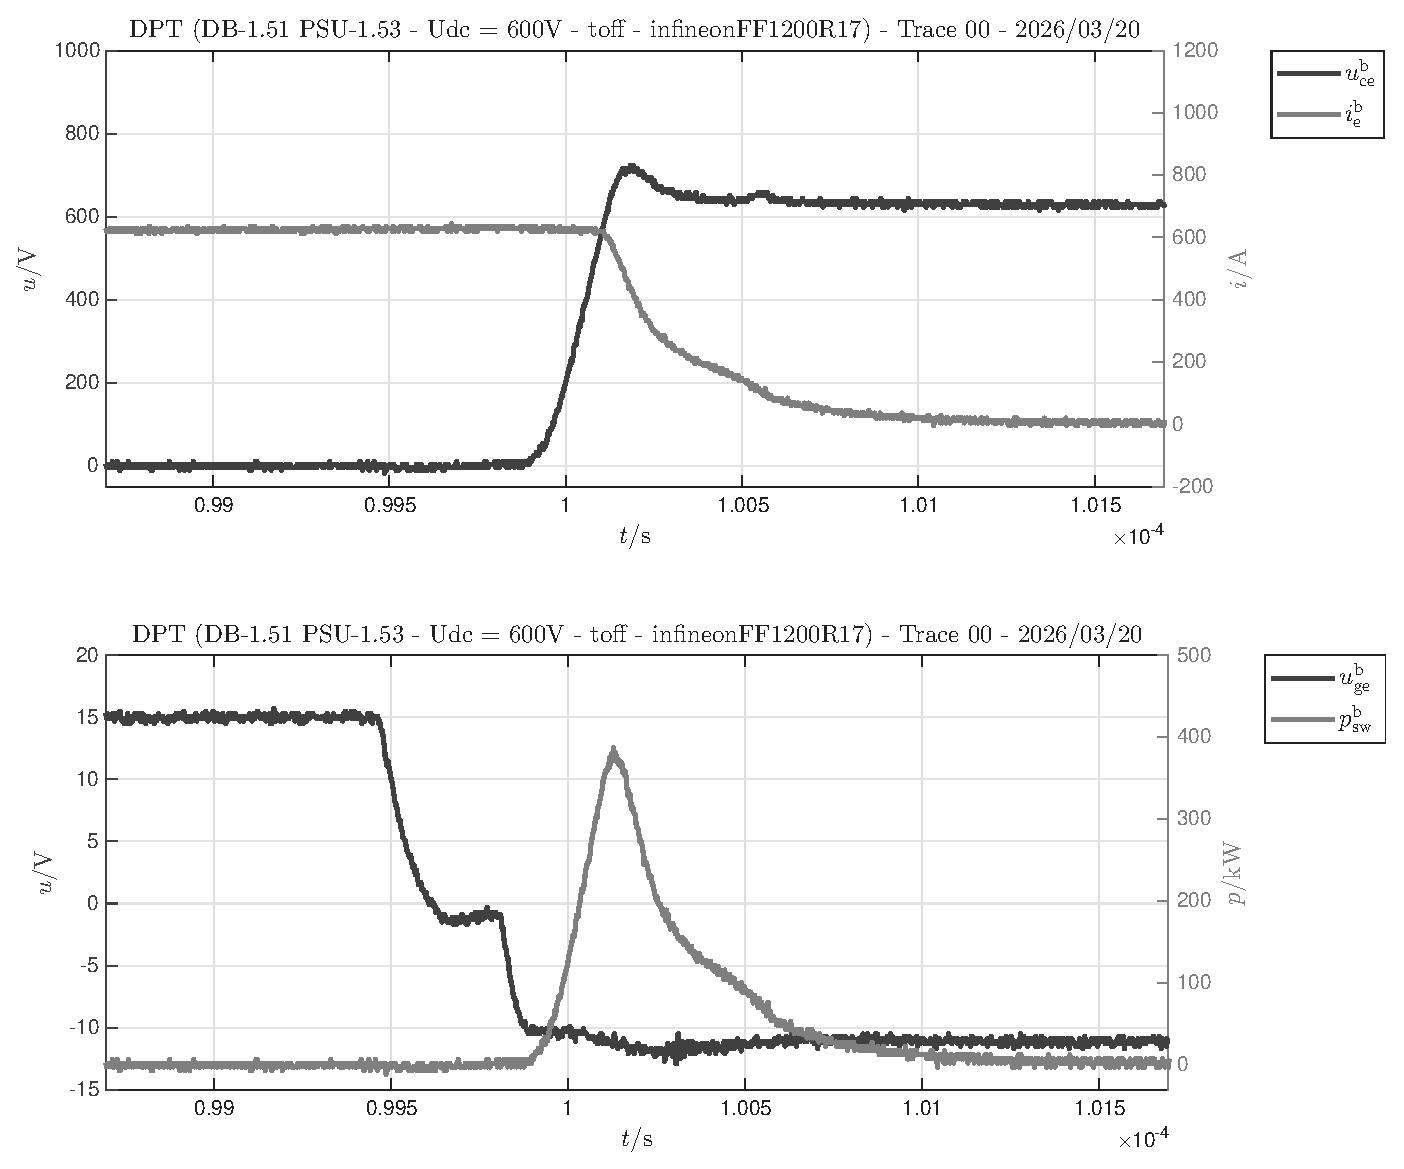
\includegraphics[width=225pt, angle=0,
				keepaspectratio]{figures/dpts/dpt_turn_off_udc600V_FF1200_DB151.eps}
				\captionsetup{width=0.65\textwidth, font=footnotesize}
				\caption{Turn-OFF: FF1200R17IP5P with DB1.51.}
				\label{fig:turn_off_FF1200_DB151_b}
			\end{subfigure}
			\captionsetup{width=0.65\textwidth, font=small}
			\caption{Turn-OFF comparison: DP650B1700 and FF1200R17IP5P with DB1.51.}
			\label{fig:turn_off_DP650_FF1200_DB151}
		\end{figure}

		\subsection{Turn-ON}
		The following waveform were acquired at the second turn-on command.\\
		
		\noindent\textbf{Remark}: DB1.00 mounts similar turn-on resistors ($R_\text{g}^\text{on}$) than DB1.51, but IGBTs turn-on with DB1.51 show a reverse recovery current ($I_\text{rr}$) slightly lower due to the presence of gate command rate limiter.\\
			
		\begin{figure}[H]
			\centering
			\begin{subfigure}{0.5\textwidth}
				\centering
				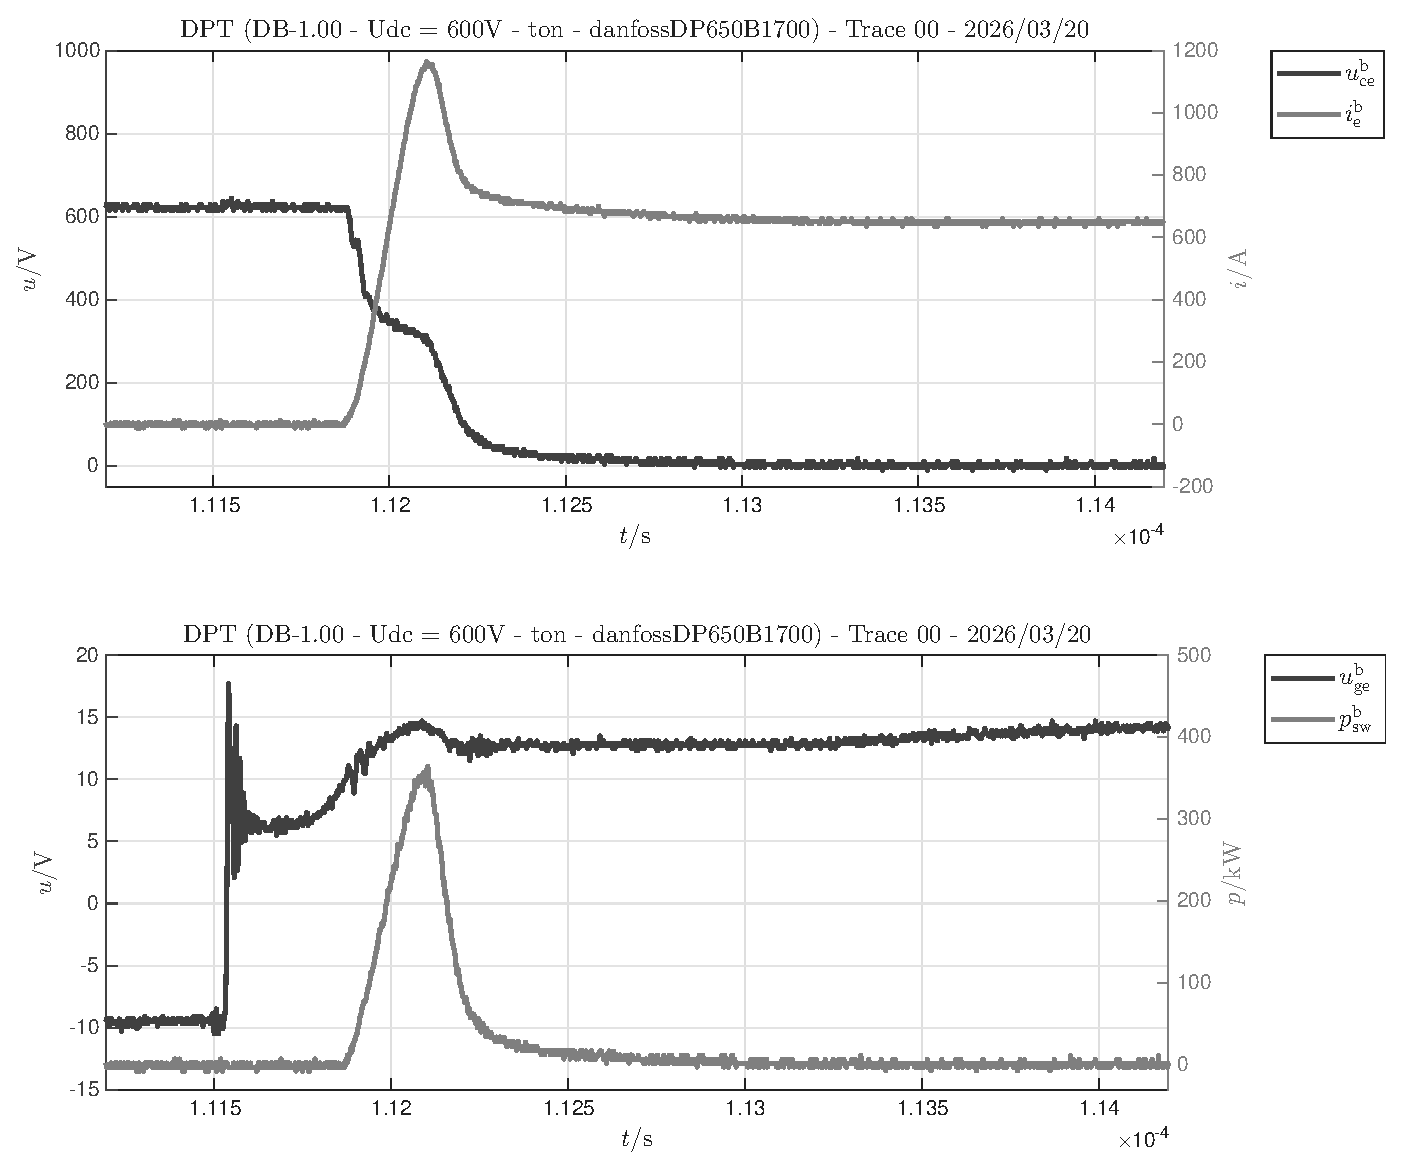
\includegraphics[width=225pt, angle=0,
				keepaspectratio]{figures/dpts/dpt_turn_on_udc600V_DP650_DB100.eps}
				\captionsetup{width=0.65\textwidth, font=footnotesize}
				\caption{Turn-ON: DP650B1700 with DB1.00.}
				\label{fig:turn_on_DP650_DB100}
			\end{subfigure}%
			\begin{subfigure}{0.5\textwidth}
				\centering
				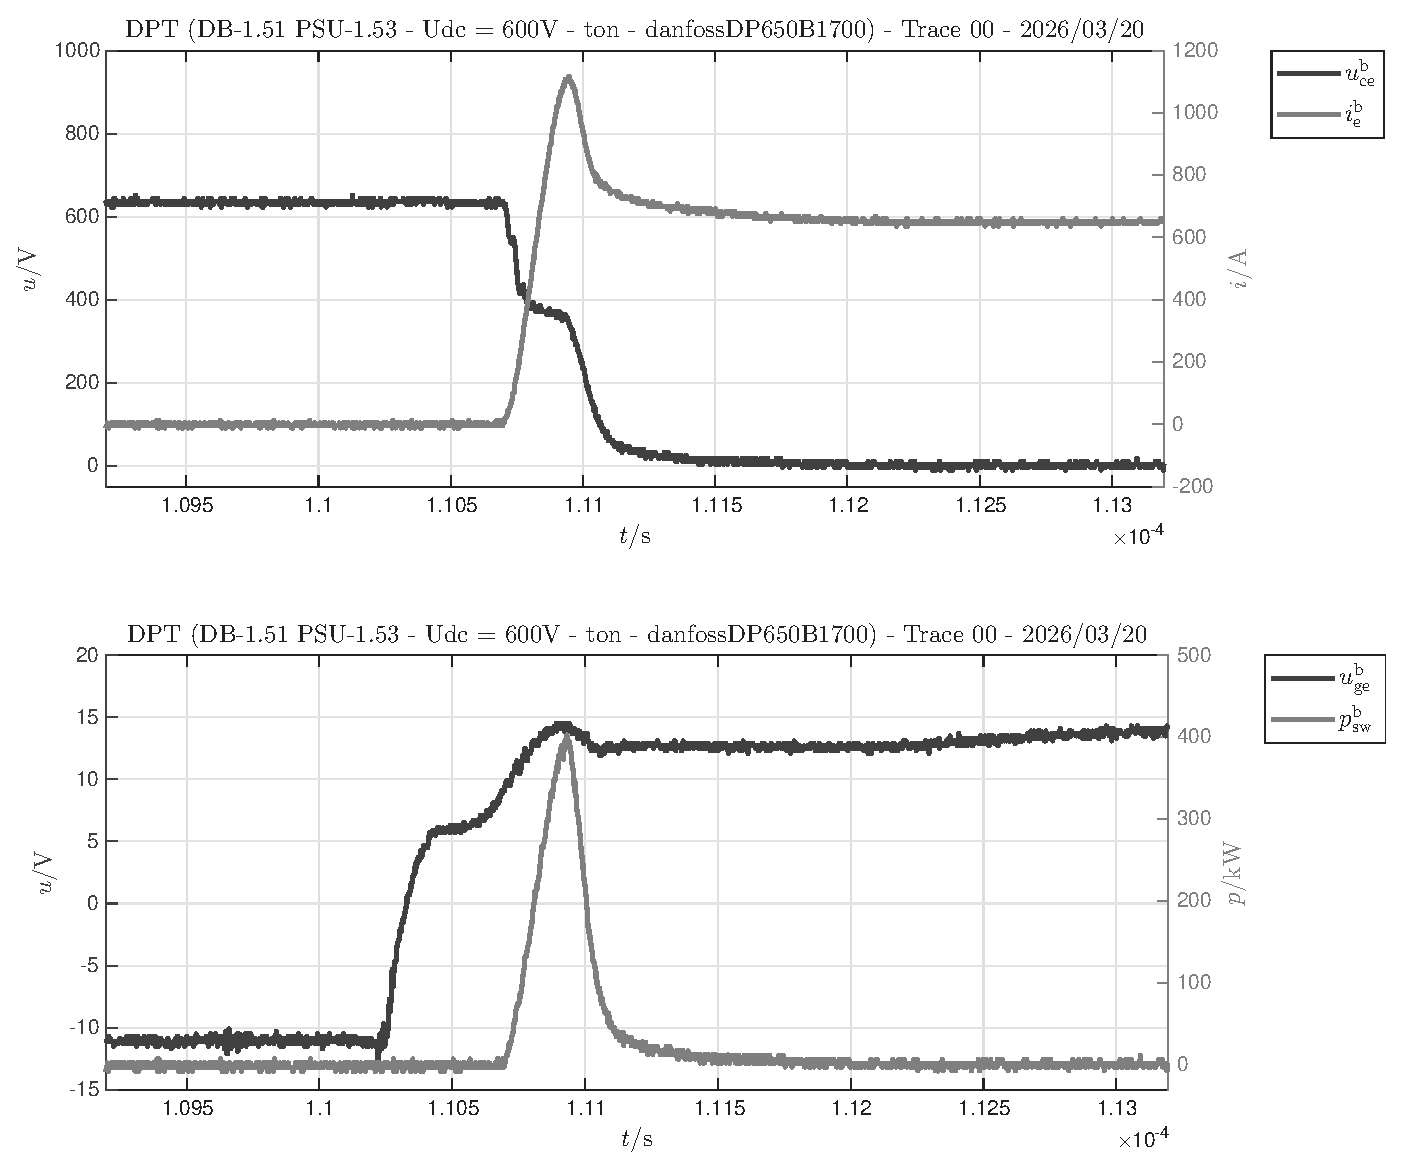
\includegraphics[width=225pt, angle=0,
				keepaspectratio]{figures/dpts/dpt_turn_on_udc600V_DP650_DB151.eps}
				\captionsetup{width=0.65\textwidth, font=footnotesize}
				\caption{Turn-ON: DP650B1700 with DB1.51.}
				\label{fig:turn_on_DP650_DB151}
			\end{subfigure}
			\captionsetup{width=0.65\textwidth, font=small}
			\caption{Turn-ON comparison: DP650B1700 with DB1.00 and DB1.51.}
			\label{fig:turn_on_DP650_DB100_DB151}
		\end{figure}

		\begin{figure}[H]
			\centering
			\begin{subfigure}{0.5\textwidth}
				\centering
				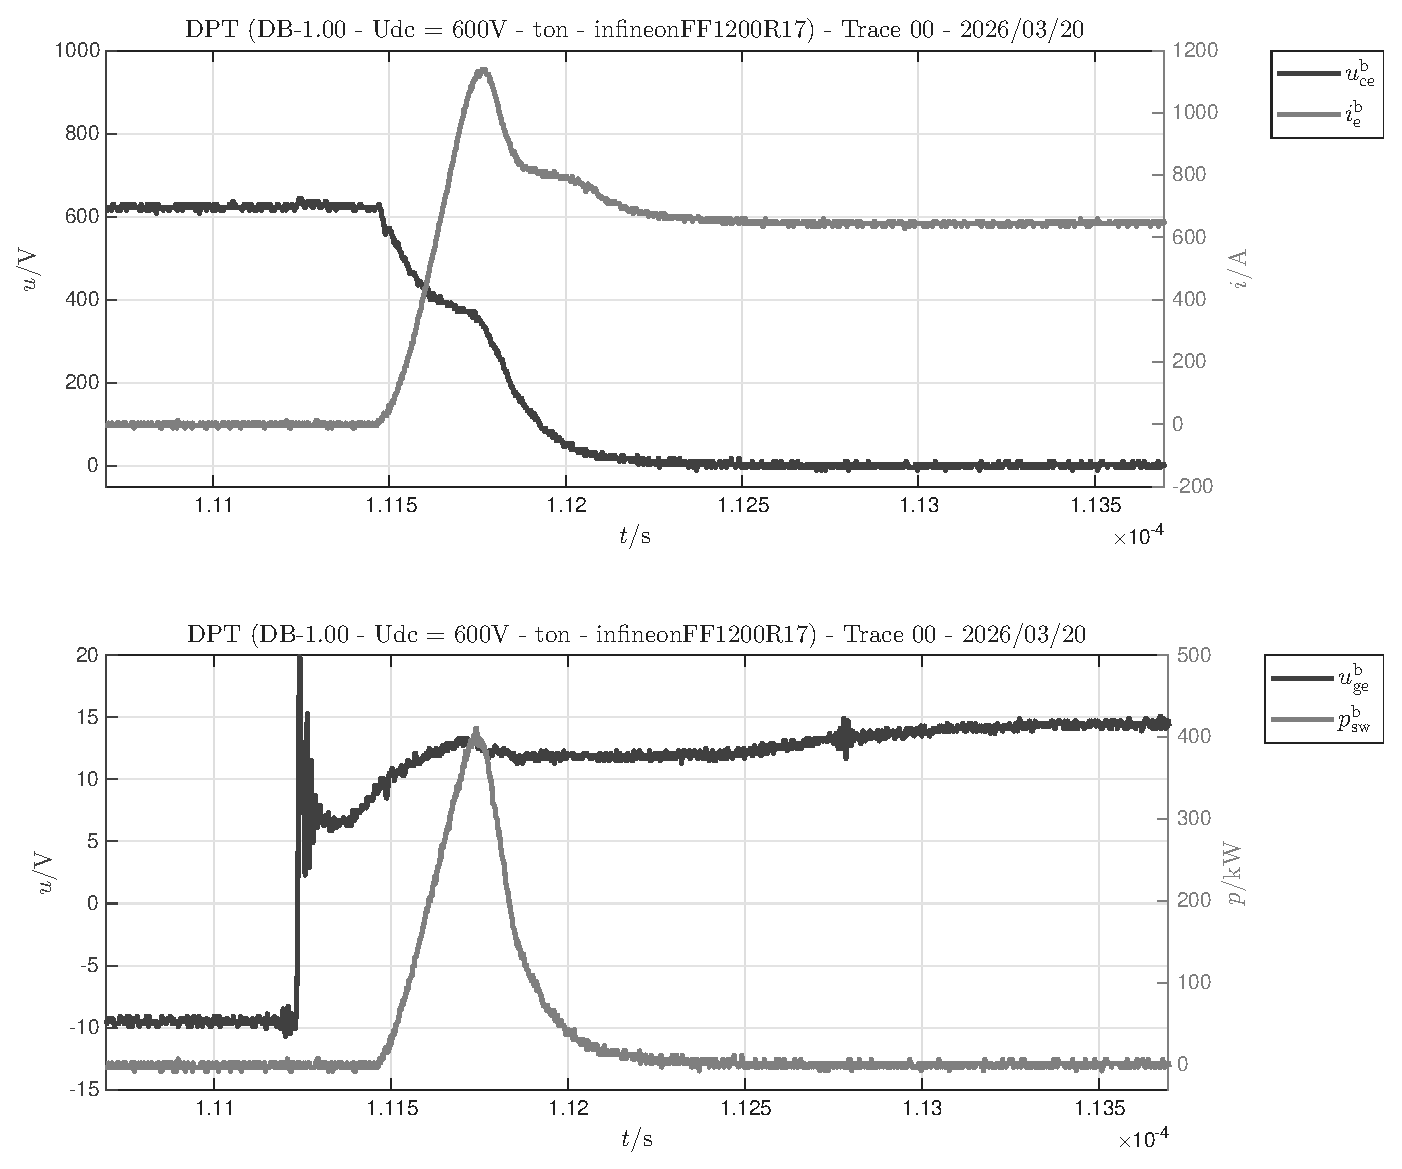
\includegraphics[width=225pt, angle=0,
				keepaspectratio]{figures/dpts/dpt_turn_on_udc600V_FF1200_DB100.eps}
				\captionsetup{width=0.65\textwidth, font=footnotesize}
				\caption{Turn-ON: FF1200R17IP5P with DB1.00.}
				\label{fig:turn_on_FF1200_DB100}
			\end{subfigure}%
			\begin{subfigure}{0.5\textwidth}
				\centering
				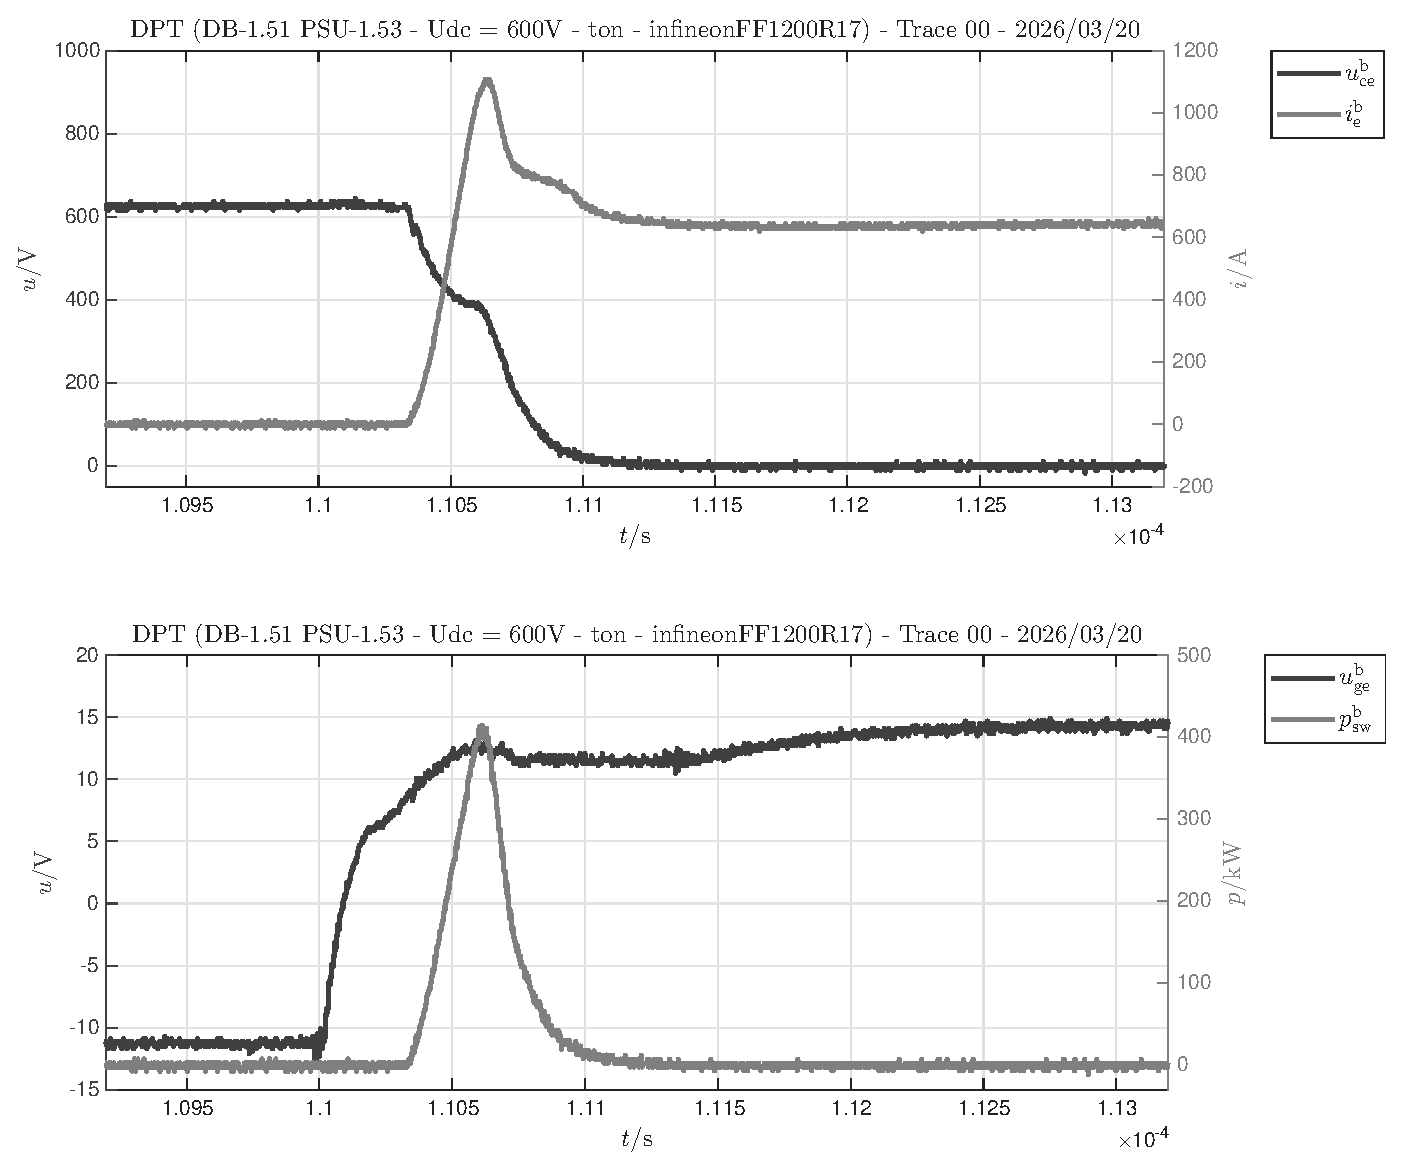
\includegraphics[width=225pt, angle=0,
				keepaspectratio]{figures/dpts/dpt_turn_on_udc600V_FF1200_DB151.eps}
				\captionsetup{width=0.65\textwidth, font=footnotesize}
				\caption{Turn-ON: FF1200R17IP5P with DB1.51.}
				\label{fig:turn_on_FF1200_DB151}
			\end{subfigure}
			\captionsetup{width=0.65\textwidth, font=small}
			\caption{Turn-ON comparison: FF1200R17IP5P with DB1.00 and DB1.51.}
			\label{fig:turn_on_FF1200_DB100_DB151}
		\end{figure}

		\begin{figure}[H]
			\centering
			\begin{subfigure}{0.5\textwidth}
				\centering
				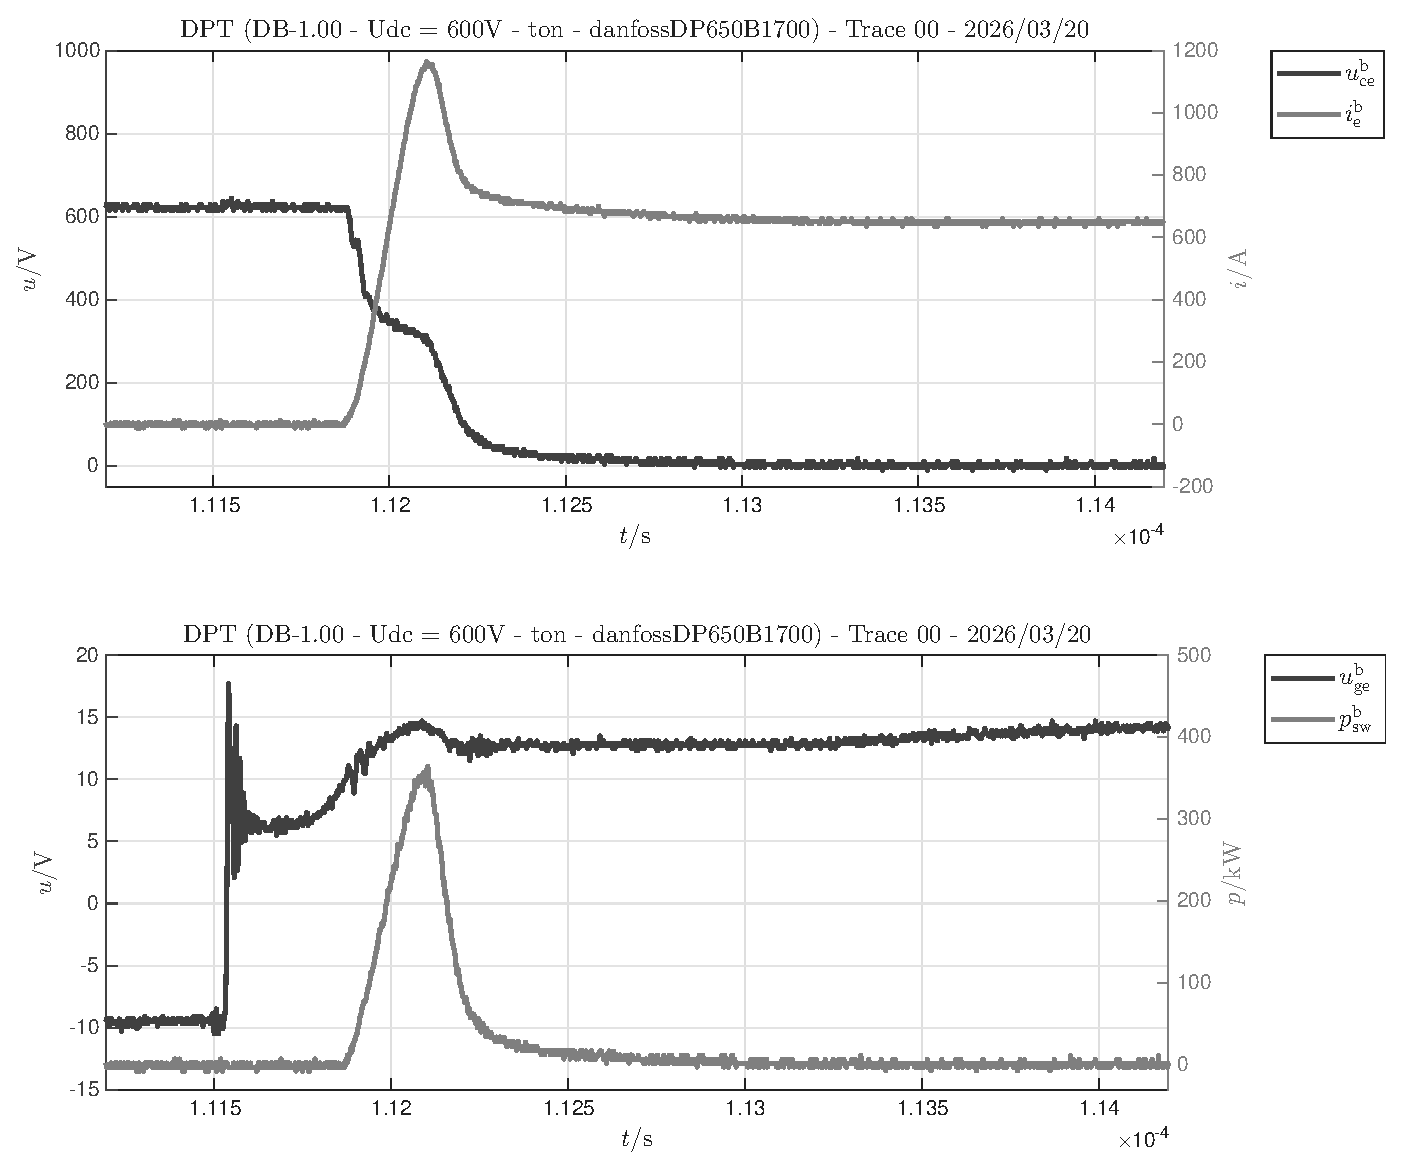
\includegraphics[width=225pt, angle=0,
				keepaspectratio]{figures/dpts/dpt_turn_on_udc600V_DP650_DB100.eps}
				\captionsetup{width=0.65\textwidth, font=footnotesize}
				\caption{Turn-ON: DP650B1700 with DB1.00.}
				\label{fig:turn_on_DP650_DB100_b}
			\end{subfigure}%
			\begin{subfigure}{0.5\textwidth}
				\centering
				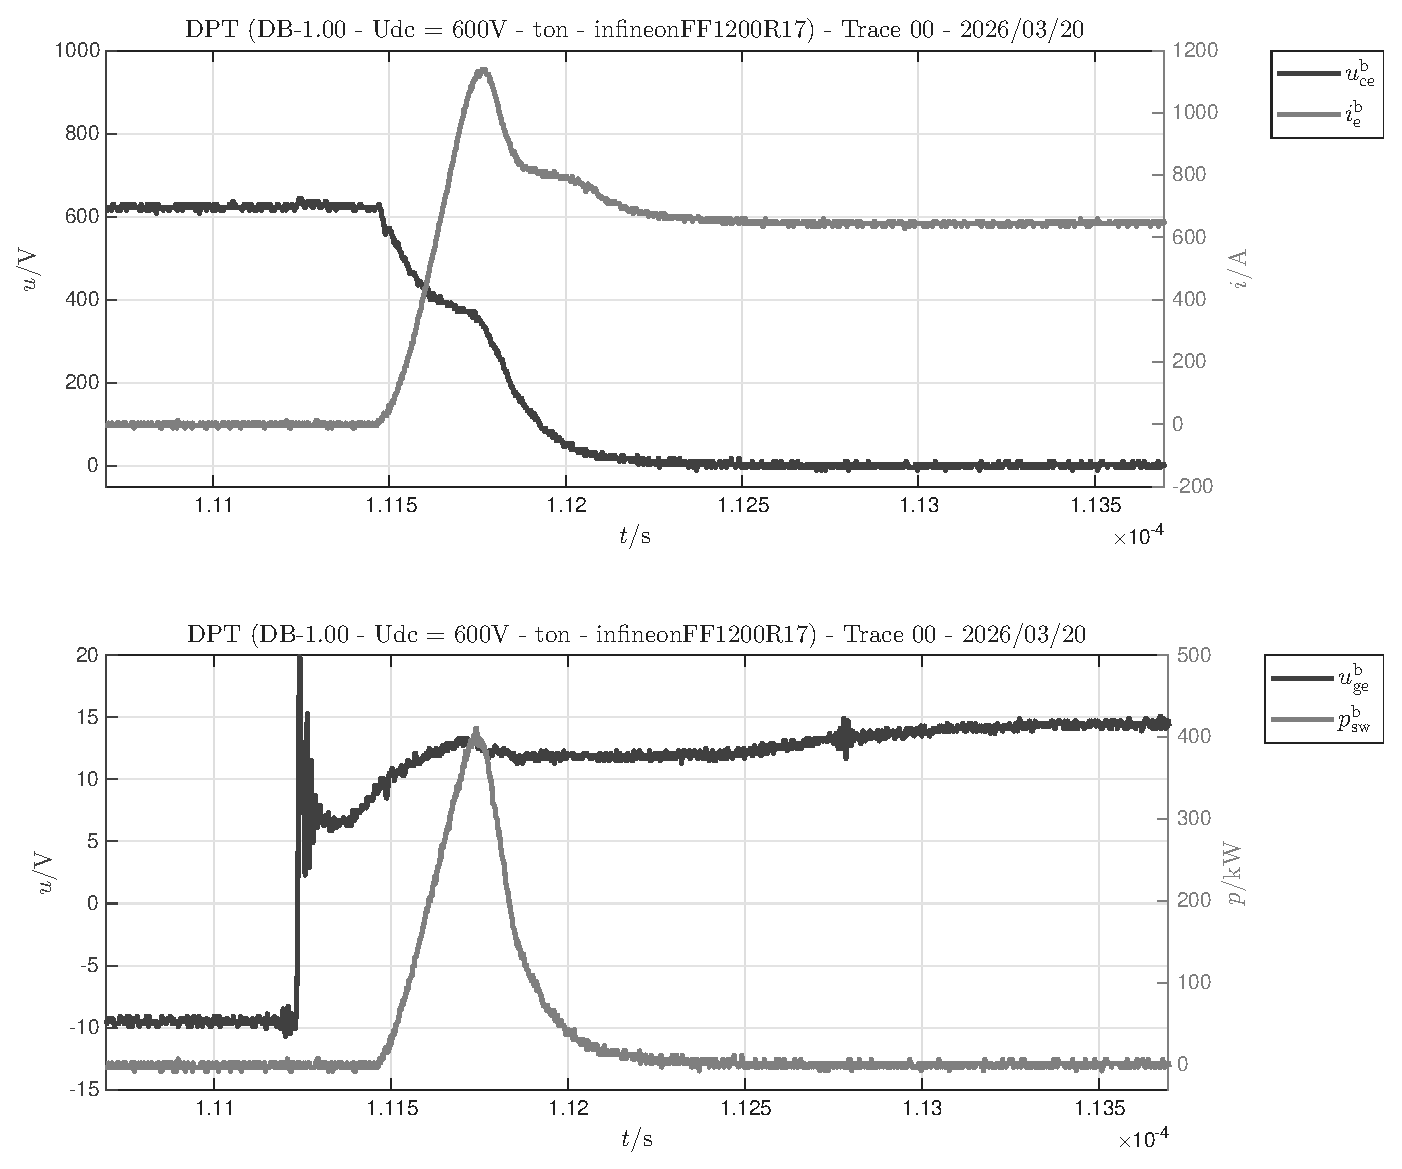
\includegraphics[width=225pt, angle=0,
				keepaspectratio]{figures/dpts/dpt_turn_on_udc600V_FF1200_DB100.eps}
				\captionsetup{width=0.65\textwidth, font=footnotesize}
				\caption{Turn-ON: FF1200R17IP5P with DB1.00.}
				\label{fig:turn_on_FF1200_DB100_b}
			\end{subfigure}
			\captionsetup{width=0.65\textwidth, font=small}
			\caption{Turn-ON comparison: DP650B1700 and FF1200R17IP5P with DB1.00.}
			\label{fig:turn_on_DP650_FF1200_DB100}
		\end{figure}

		\begin{figure}[H]
			\centering
			\begin{subfigure}{0.5\textwidth}
				\centering
				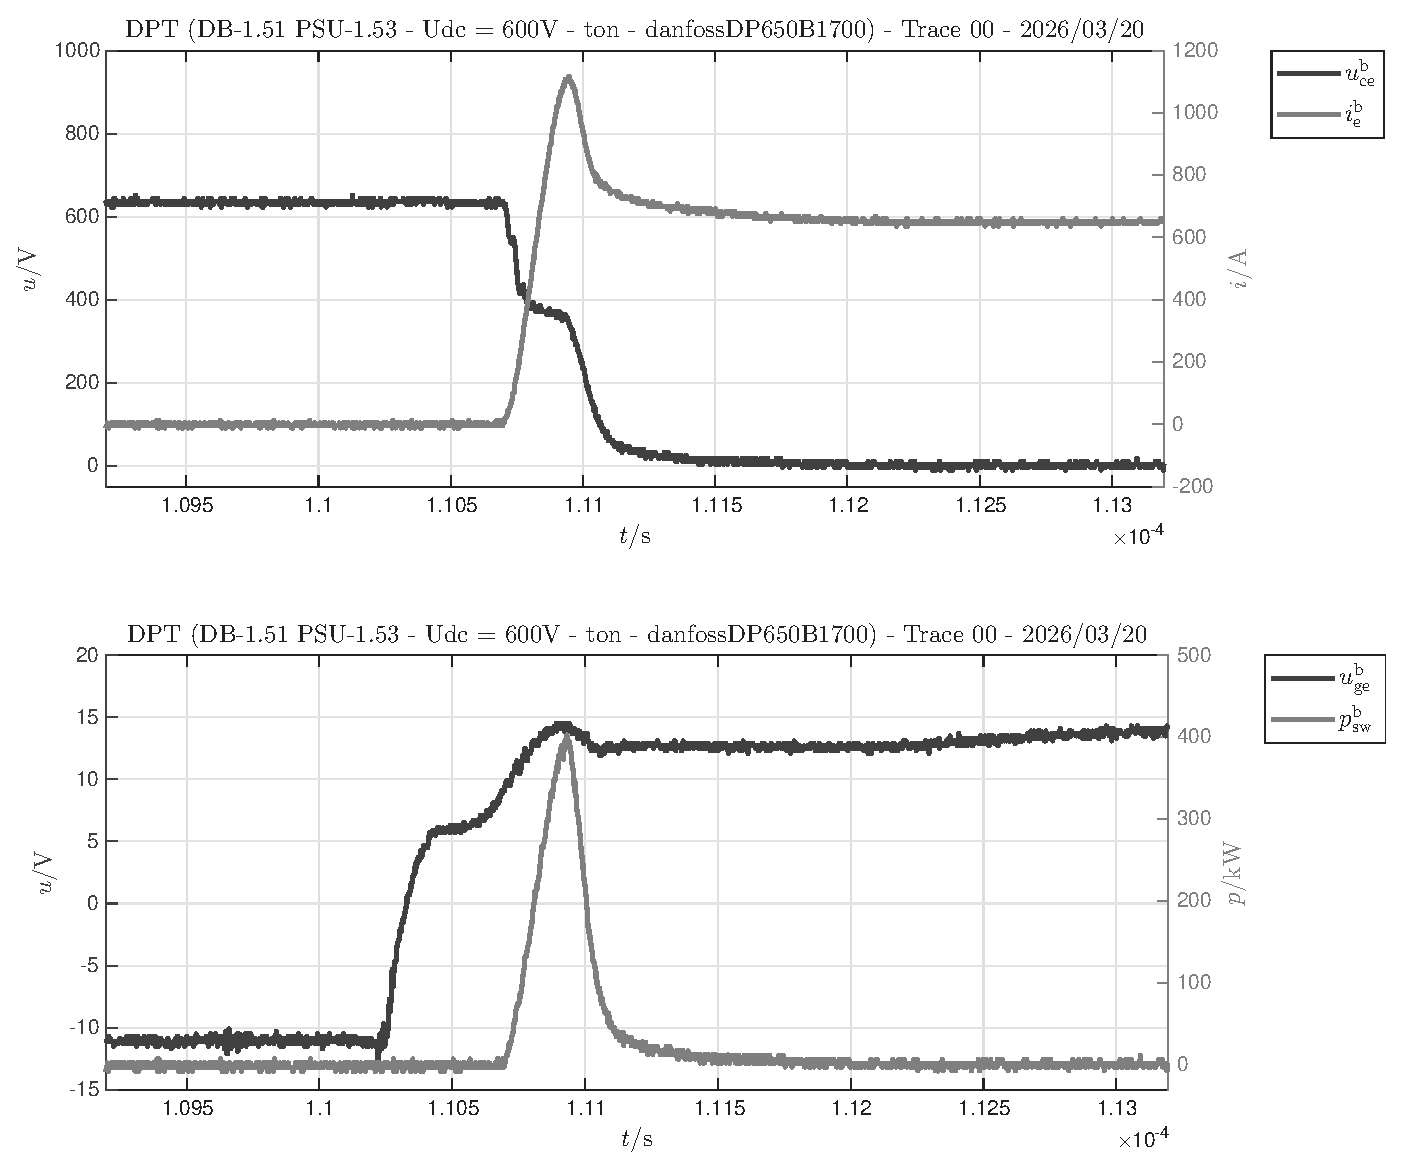
\includegraphics[width=225pt, angle=0,
				keepaspectratio]{figures/dpts/dpt_turn_on_udc600V_DP650_DB151.eps}
				\captionsetup{width=0.65\textwidth, font=footnotesize}
				\caption{Turn-ON: DP650B1700 with DB1.51.}
				\label{fig:turn_on_DP650_DB151_b}
			\end{subfigure}%
			\begin{subfigure}{0.5\textwidth}
				\centering
				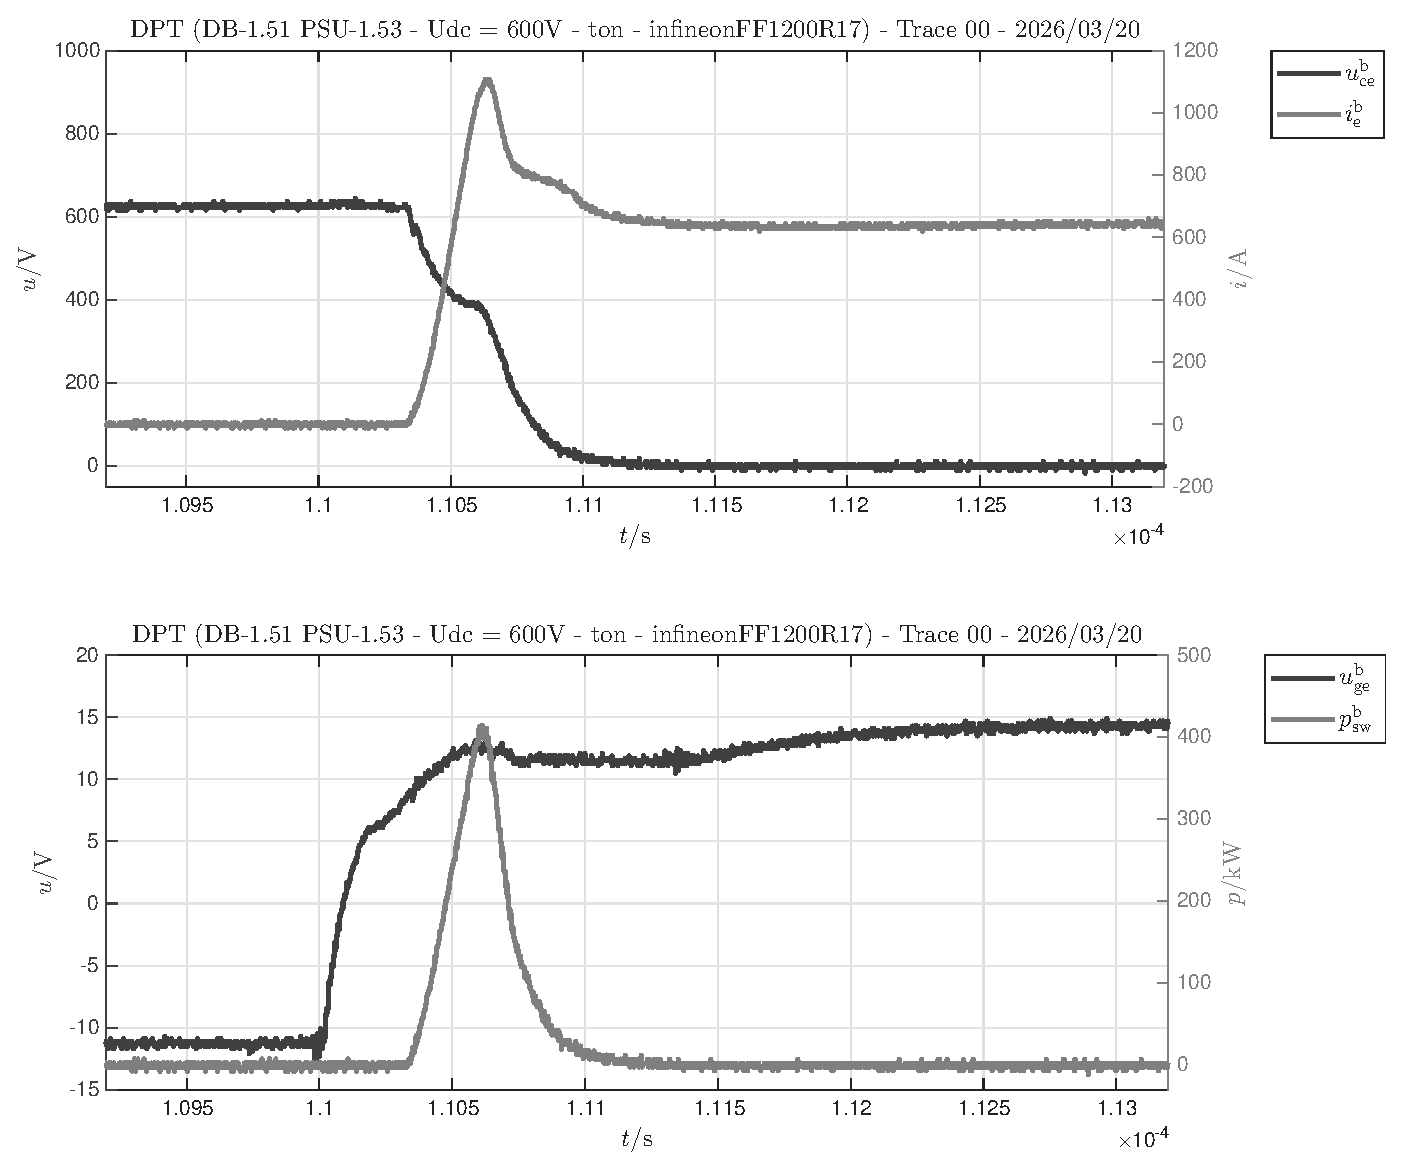
\includegraphics[width=225pt, angle=0,
				keepaspectratio]{figures/dpts/dpt_turn_on_udc600V_FF1200_DB151.eps}
				\captionsetup{width=0.65\textwidth, font=footnotesize}
				\caption{Turn-ON: FF1200R17IP5P with DB1.51.}
				\label{fig:turn_on_FF1200_DB151_b}
			\end{subfigure}
			\captionsetup{width=0.65\textwidth, font=small}
			\caption{Turn-ON comparison: DP650B1700 and FF1200R17IP5P with DB1.51.}
			\label{fig:turn_on_DP650_FF1200_DB151}
		\end{figure}

		\newpage
		\subsection{Summary of Test Results}
		The tests were carried out under the four configurations defined in
		Section~\ref{sec:scope}, repeated here for convenience:
		\begin{itemize}
			\item[--] \textbf{Case\,1}: DP650B1700 with DB1.00;
				\begin{itemize}
					\item[--] series-production IGBT module with series-production driver board;
				\end{itemize}
			\item[--] \textbf{Case\,2}: DP650B1700 with DB1.51;
				\begin{itemize}
					\item[--] series-production IGBT module with candidate driver board;
				\end{itemize}
			\item[--] \textbf{Case\,3}: FF1200R17IP5P with DB1.00;
				\begin{itemize}
					\item[--] candidate IGBT module with series-production driver board;
				\end{itemize}
			\item[--] \textbf{Case\,4}: FF1200R17IP5P with DB1.51;
				\begin{itemize}
					\item[--] candidate IGBT module with candidate driver board.
				\end{itemize}
		\end{itemize}
		The main results are summarised in Table~\ref{summary_results_table_1}.

		\begin{table}[h]
			\centering
			\captionsetup{width=0.75\textwidth, font=small}
			\caption{Summary of DPT results.}
			\label{summary_results_table_1}
			\renewcommand{\arraystretch}{2.0}
			\begin{tabularx}{0.75\textwidth}{X|>{\centering\arraybackslash}X|>{\centering\arraybackslash}X|>
					{\centering\arraybackslash}X|>{\centering\arraybackslash}X}
				\hline\hline
				& \textbf{Case\,1} & \textbf{Case\,2} & \textbf{Case\,3} & \textbf{Case\,4} \\
				\hline
				$E_\text{on}$\,$\left[\si{\milli\joule}\right]$  & 80  & 91  & 105 & 107 \\
				\hline
				$E_\text{off}$\,$\left[\si{\milli\joule}\right]$ & 90  & 93  & 152 & 130 \\
				\hline
				$I_\text{rr}$\,$\left[\si{\ampere}\right]$       & 512 & 448 & 488 & 464 \\
				\hline
				$\Delta u_\text{ce}$\,$\left[\si{\volt}\right]$  & 245 & 187 & 173 & 86  \\
				\hline\hline
			\end{tabularx}
		\end{table}

		\noindent\textbf{Remark} --- The gate resistances mounted on the two driver boards are as follows:
		\begin{equation}
			\begin{aligned}
				&R_\text{g}^\text{on}\,\Big|_{\text{DB1.00}} = \frac{\SI{6.2}{\ohm}}{5} = \SI{1.24}{\ohm}, \qquad
				R_\text{g}^\text{off}\,\Big|_{\text{DB1.00}} = \frac{\SI{18.0}{\ohm}}{5} = \SI{3.6}{\ohm} \\[6pt]
				&R_\text{g}^\text{on}\,\Big|_{\text{DB1.51}} = \frac{\SI{4.47}{\ohm}}{4} = \SI{1.175}{\ohm}, \qquad
				R_\text{g}^\text{off}\,\Big|_{\text{DB1.51}} = \frac{\SI{4.47}{\ohm}}{4} = \SI{1.175}{\ohm}
			\end{aligned}
		\end{equation}

		\newpage
		The reference data shown in Table~\ref{tab:reference_energies} have been scaled from the
		device datasheets, accounting for collector current $I_\text{c}$, collector-emitter
		voltage $V_\text{ce}$, and case temperature $T_\text{case}$ (assumed equal to the
		junction temperature) using simple linear scaling.

		DPTs were carried out at $I_\text{c} = \SI{620}{\ampere}$ and
		$V_\text{ce} = \SI{630}{\volt}$, yielding the following reference switching energy values:

		\begin{table}[h]
			\centering
			\captionsetup{width=0.75\textwidth, font=small}
			\caption{Reference $E_\text{on}$ and $E_\text{off}$ for the DPTs.}
			\label{tab:reference_energies}
			\renewcommand{\arraystretch}{2.0}
			\begin{tabularx}{\textwidth}{Y|Z|Z|Z|Z|Z|Z|Z}
				\hline\hline
				& $T_\text{case}$ & $E_\text{on}^\text{ref}$ & $E_\text{off}^\text{ref}$ & $I_\text{c}$ & $V_\text{ce}$ & $R_\text{g}^\text{on}$ & $R_\text{g}^\text{off}$ \\
				\hline
				FF650R17IE4  & \SI{25}{\celsius} & \SI{136}{\milli\joule} & \SI{93}{\milli\joule}  & \SI{620}{\ampere} & \SI{630}{\volt} & \SI{1.24}{\ohm}   & \SI{3.6}{\ohm}   \\
				\hline
				FF1200R17IP5P & \SI{25}{\celsius} & \SI{132}{\milli\joule} & \SI{100}{\milli\joule} & \SI{620}{\ampere} & \SI{630}{\volt} & \SI{1.175}{\ohm}  & \SI{1.175}{\ohm} \\
				\hline\hline
			\end{tabularx}
		\end{table}

		\begin{table}[h]
			\centering
			\captionsetup{width=0.75\textwidth, font=small}
			\caption{Measured $E_\text{on}$ and $E_\text{off}$ with DB1.51.}
			\label{tab:measured_energies_DB151}
			\renewcommand{\arraystretch}{2.0}
			\begin{tabularx}{\textwidth}{Y|Z|Z|Z|Z|Z|Z|Z}
				\hline\hline
				& $T_\text{case}$ & $E_\text{on}^\text{m}$ & $E_\text{off}^\text{m}$ & $I_\text{c}$ & $V_\text{ce}$ & $R_\text{g}^\text{on}$ & $R_\text{g}^\text{off}$ \\
				\hline
				FF650R17IE4   & \SI{25}{\celsius} & \SI{91}{\milli\joule}  & \SI{93}{\milli\joule}  & \SI{620}{\ampere} & \SI{630}{\volt} & \SI{1.175}{\ohm} & \SI{1.175}{\ohm} \\
				\hline
				FF1200R17IP5P & \SI{25}{\celsius} & \SI{107}{\milli\joule} & \SI{130}{\milli\joule} & \SI{620}{\ampere} & \SI{630}{\volt} & \SI{1.175}{\ohm} & \SI{1.175}{\ohm} \\
				\hline\hline
			\end{tabularx}
		\end{table}

		\begin{table}[h]
			\centering
			\captionsetup{width=0.75\textwidth, font=small}
			\caption{Measured $E_\text{on}$ and $E_\text{off}$ with DB1.00.}
			\label{tab:measured_energies_DB100}
			\renewcommand{\arraystretch}{2.0}
			\begin{tabularx}{\textwidth}{Y|Z|Z|Z|Z|Z|Z|Z}
				\hline\hline
				& $T_\text{case}$ & $E_\text{on}^\text{m}$ & $E_\text{off}^\text{m}$ & $I_\text{c}$ & $V_\text{ce}$ & $R_\text{g}^\text{on}$ & $R_\text{g}^\text{off}$ \\
				\hline
				FF650R17IE4   & \SI{25}{\celsius} & \SI{80}{\milli\joule}  & \SI{90}{\milli\joule}  & \SI{620}{\ampere} & \SI{630}{\volt} & \SI{1.24}{\ohm} & \SI{3.6}{\ohm} \\
				\hline
				FF1200R17IP5P & \SI{25}{\celsius} & \SI{105}{\milli\joule} & \SI{152}{\milli\joule} & \SI{620}{\ampere} & \SI{630}{\volt} & \SI{1.24}{\ohm} & \SI{3.6}{\ohm} \\
				\hline\hline
			\end{tabularx}
		\end{table}
	
		\noindent\textbf{Remark}: The new IGBT module FF1200R17IP5P exhibits higher switching power losses compared to the other modules under the same load conditions; however, it demonstrates superior performance in terms of conduction power losses. Furthermore, the FF1200R17IP5P features a lower thermal impedance, resulting in more efficient thermal energy dissipation. As a consequence, the maximum junction temperature is approximately \SI{15}{\celsius} lower than that of the other modules. It is worth noting that this device is rated for a maximum junction temperature of \SI{175}{\celsius}, whereas the remaining modules are rated at \SI{150}{\celsius}, providing an additional thermal safety margin.
	
		\section{Overall Results and Conclusions}
		Based on the data collected in the previous sections, the FF1200R17IP5P module in
		combination with the DB1.51 driver board demonstrates full compatibility and satisfies
		all design requirements. It is therefore recommended to proceed with further
		investigations, including load testing, to validate the module under real operating
		conditions.

	\end{onehalfspace}
	
	\newpage
	\begin{thebibliography}{99}
		\bibitem{holm} 
		D. A. Neamen \emph{Semiconductor Physiscs and Devices}. Springer-Verlag. McGraw Hill, Fourth Edition 2012.
	\end{thebibliography}
\end{document}
